\newtheorem{definition}{Definícia}[section]
\newtheorem{example}{Príklad}[section]

\def\UrlBreaks{\do\/\do-}

\chapter{Úvod}
Formálne modely nám vedia sprostredkovať teoretické prostriedky pre popis rôznych praktických aplikácií. Najväčšou aplikáciou z nich sú programovacie jazyky a dizajn prekladačov týchto jazykov. Ďalšie aplikácie vieme nájsť v biológii, lingvistike alebo umení. Cieľom tejto práce je aplikácia formálnych modelov v umení, konkrétne v hudbe.

Hudobná štruktúra, na ktorú sú aplikované formálne modely v tejto práci sa nazýva téma a variácie. Väčšina moderných i klasických skladieb sa neskladá z čisto nových tónov a úsekov. Množstvo úsekov sa opakuje, ale nie vždy v ich rovnakom znení. Tieto opakovania sú obmieňané rôznymi spôsobmi. Tieto spôsoby môžu byť zmena rytmu, melódie alebo tóniny. Súčasťou tejto práce je zistiť ako môžeme popísať tieto štruktúry. Prípadne nájsť riešenie, ktoré ponúka ich tvorbu.

Za hudbu môžeme považovať štruktúru, ktorá sa riadi určitými pravidlami. Napriek tomu, že obsahuje množstvo pravidiel a predpisov, je to prostriedok pre vyjadrenie myšlienky skladateľa. Táto myšlienka odzrkadľuje nálady, prostredie alebo zážitky skladateľa. Takže sa neriadi žiadnymi deterministickými pravidlami. Hlavná myšlienka, ktorá sa nazýva téma je konečná množina tónov, ktoré sú podľa ich dĺžky začlenené do taktov. Obsahom hudby nie je čisto len téma, ale obsahuje aj jej obmieňanie rôznymi hudobnými prostriedkami. Prepojením takýchto štruktúr vzniká celá skladba, ktorá sa skladá z témy a jej variácií. Príkladom takejto skladby môže byť Dvanásť variácií na \uv{Ah vous dirai-je, Maman}. Vzniknutá skladba je štruktúra, ktorá sa skladá z témy a variácie. Cieľom tejto práce je popísanie tejto štruktúry vhodným formálnym modelom. Výsledkom tohto popisu by malo byť stvárnenie týchto štruktúr, ktoré nesmie obmedzovať tvorbu hudby.

V prípade navrhnutého správneho modelu, ktorý by vedel popisovať túto hudobnú štruktúru, je súčasťou práce ho aplikovať. Ako najvhodnejšia aplikácia, ktorá sa dá v hudbe nájsť je jej tvorba. Gramatiky, ktoré sú súčasťou formálnych modelov umožňujú generovať rôzne reťazce. Preto predmetom aplikácie je vytvoriť gramatiku, ktorá tvorí hudobné reťazce, ktoré by zároveň dávali hudobný zmysel. Na vytvorenie takýchto reťazcov je potrebná gramatika, ktorá vie zvládnuť tvorbu týchto reťazcov. Preto je potrebné zaradiť hudbobný jazyk do jeho príslušnej triedy v Chomského hierarchie. Zistenie triedy takéhoto jazyka vedie k odhadu gramatiky, ktorá by mohla takýto reťazce generovať. 

Text tejto práce je rozdelený do viacerých sekcii. Kapitola \ref{chap:definitions} sa skladá z dvoch sekcií. Sekcia \ref{sec:music} sa zaoberá základnými pojmami v hudbe, ktorá vedie k pochopeniu použitej hudobnej terminologie. Sekcia \ref{sec:formallang} rozoberá jazyky Chomského hierarchie. Ďalej rozoberá, do ktorej kategórie je zaradený jazyk pre popis témy a variácii. V kapitole \ref{chap:app} definujeme gramatiku, ktorá bola použitá pre popis hudobnej štruktúry. Spolu s definíciou nového modelu ukazuje jeho aplikácie pre hudobnú štruktúru. Kapitola \ref{chap:imp} sa venuje samotnej implementácii novej verzie modelu, spusteniu tejto implementácii a ukážkami výsledku tejto implementácie. Posledná kapitola \ref{chap:end} vyhodnocuje výsledky práce, poukazuje na ich praktické použitie. Obsahom tejto kapitoly je aj diskusia k ďalšiemu pokračovaniu tejto práce. 


\chapter{Základné pojmy a definície}
\label{chap:definitions}
Táto kapitola oboznamuje so základnými pojmami, ktoré vedú k pochopeniu obsahu tejto bakalárskej práce. Vzhľadom na to, že táto práca je úzko spätá s hudbou a hudobnou teóriou, obsahuje jej základy, ktoré sú prevzaté z \cite{MUSICTHEORY, DunnettVar}. Základy formálných jazykov a ich definície sú prevzaté z \cite{MEDUNATHEORY}.

\section{Hudba}
\label{sec:music}
Hudba je súčasťou umenia. Základným stavebným materiálom hudby je tón. Pomocou hudby sa skladateľ snaží vyjadriť nejakú myšlienku. Hudobnú myšlienku je možné zapísať notami pomocou notového zápisu. Cieľom tejto podkapitoly je objasnenie základných pojmov hudby, ako i ukážka hudobnej štruktúry téma a variácie.

\subsection{Tón}
Tón je definovaný, ako zvuk s určitou výškou a vzniká pravidelným chvením nejakého zdroja zvuku. Vzniknuté chvenie sa prenáša do sluchových orgánov zmenou hustoty vzduchu. Skladá sa z rôznych vlastností, ako sú výška, sila, farba a dĺžka. Najdôležitejšie vlastnosti sú výška tónu a jeho dĺžka, ktoré sú predmetom tejto práce.

Dĺžka tónu nie je narozdiel od ostatných vlastností fyzikálnou, ale je závislá od interpreta daného tónu. Čas znejúceho tonu je jeho dĺžkou. Interpret jeho zásahom pri interpretácií vie určiť dĺžku tónu. Interpretom je v našej práci program. Dĺžka tónu je vopred definovaná.

Výška tónu je definovaná ako počet kmitov za jednu sekundu. Spolu s výškou tónu sa zvyšuje počet kmitov za sekundu. Počet kmitov za jednu sekundu sa udáva v Hertzoch.

Tóny sú usporiadané do tónovej sústavy. Tónová sústava je množina tónov, ktoré sa v hudbe vyskytujú. Tvorí ju sedem základných tónov c, d, e, f, g, a, h. Tieto tóny sú výškovo usporiadané od najnižšej po najvyššiu. Po tóne h vždy nasleduje tón c, ktorý má dvojnásobnú frekvenciu oproti tomu pôvodnému. Všetkých osem tónov tvorí oktávu. V tejto práci sú použité dve oktávy, a to sú jednočiarkovaná oktáva a dvojčiarkovaná oktáva.

Na obrázku \ref{fig:tonfrek} sú zobrazené tóny cez dve oktávy, ktoré sú pomenované. K príslušným tónom bola priradená ich frekvencia na základe \cite{strankaFrekvencii}. Na obrázku môžeme spozorovať, ako frekvencie tónov medzi oktávami súvisia. Jednočiarkovaná oktáva, ktorá sa začína tónom c a končí tónom c2 má polovičnú frekvenciu dvojčiarkovanej oktávy, ktorá sa začína tónom c2 a končí tónom c3. Jednotlivé tóny vieme posunúť o oktávu vyššie vďaka znásobeniu ich frekvencie.

\begin{figure}[H]
\centering
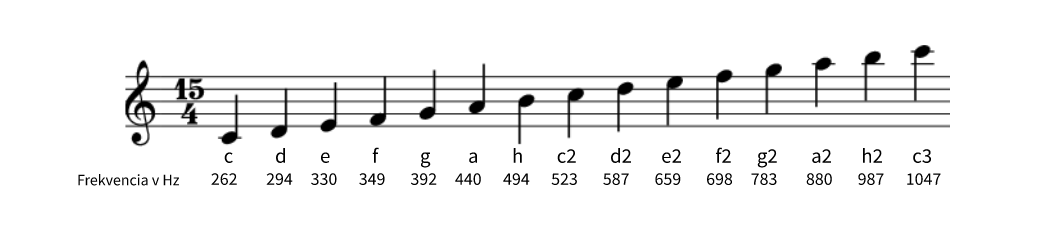
\includegraphics[scale=0.4]{obrazky-figures/Tonyafrekvencie.png}
\caption{Postupnosť tónovov cez dve oktávy s príslušnými frekvenciami.}
\label{fig:tonfrek}
\end{figure}

\subsection{Nota}
\label{subs:nota}
Nota je grafická značka, ktorá sa zapisuje do notovej osnovy. Pomocou noty vieme vyjadriť dĺžku tónu a jeho výšku. Ostatné vlastnosti tónu sa zapisujú inými značkami. Zápis nôt do notovej osnovy je potrebný pre reprezentáciu hudobnej myšlienky alebo jej interpretáciu. Noty majú rôzne značenie. Notu tvorí hlavička a nožička. V tejto práci sú použité štyri základné značenia, ako sú celá nota, polová nota, štvrťová nota a osminová nota. Tieto notové značenia sú na obrázku \ref{fig:druhnot}.

\begin{figure}[H]
\centering
\includegraphics[scale=0.4]{obrazky-figures/Druhynôt.png}
\caption{Notové značenia.}
\label{fig:druhnot}
\end{figure}

\subsection{Takt}
Pod taktom v hudbe rozumieme základnú jednotku pravidelného striedania prízvučných a neprízvučných dôb. Určuje sa v notovom zápise, na začiatku skladby. Značený je dvomi číslami. Vrchné číslo určuje počet dôb v jednom takte. Spodné číslo označuje notu, ktorá trvá jednu dobu.

Na obrázku \ref{fig:dvojst} je dvojštvrťový takt, ktorý obsahuje dve štvrťové noty c, d. Dvojka značí to, že v jednom takte sa môžu maximálne vyskytovať dve doby. Štvorka označuje trvanie štvrťovej noty, ktorá trvá jednu dobu. V tomto takte sa nemôže napríklad vyskytovať celá nota, ktorá trvá štyri doby a presahuje tak dĺžku jedného taktu.

\begin{figure}[H]
\centering
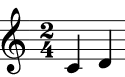
\includegraphics[scale=0.4]{obrazky-figures/dvojst.png}
\caption{Dvojštvrťový takt.}
\label{fig:dvojst}
\end{figure}


Obrázok \ref{fig:trojst} už obsahuje štvorštvrťový takt, v ktorom sa už môže vyskytovať celá nota, ktorá trvá štyri doby.

\begin{figure}[H]
\centering
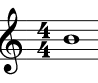
\includegraphics[scale=0.4]{obrazky-figures/cela.png}
\caption{Štvorštvrťový takt.}
\label{fig:trojst}
\end{figure}

\subsection{Notový zápis}
Notový zápis sa skladá z piatich čiar a štyroch medzier. Začína sa klúčom, ktorý slúži pre relatívne určenie výšky skladby. Existujú rôzne kľúče. V tejto práci sa vyskytuje jeden a tým je husľový kľúč. Husľovým kľúčom sa zapisujú tóny stredné a vysoké. 

Po husľovom kľúči sa určí tónina. Tónina je množina tónov, ktorá je obsiahnutá v melódií. Každá tónina prislúcha nejakej stupnici. Stupnicu tvorí osem základných tónov, ktoré sú výškovo usporiadané. Stupnica sa začína tónom, ktorý prisluši názvu stupnici. C durová stupnica sa začína tónom c. V tejto práci sa pracuje čisto s notami z C durovej stupnice a výsledky práce sú v C durovej tónine.

Zapísaný kľúč a tóninu, v ktorej je melódia zapísaná nasleduje určenie taktového predpisu. Posledná časť notového zápisu je samotná melódia, ktorá je zapísaná notami.

V prípade, že k zápisu nôt do notovej osnovy nestačí počet čiar, potom sa pridávajú pomocné čiary. Príklad pomocnej čiary je pre notu c na obrázku \ref{fig:tonfrek}.

\subsection{Téma a variacie}
Téma a variácie sú bežné hudobné prostriedky, ktoré tvoria hudobnú štruktúru. Táto hudobná štruktúra je používaná vo veľkej miere v klasickej hudbe. Štruktúra je založená na téme, ktorá sa vyskytuje na začiatku hudobnej myšlienky. Potom, ako odznie téma prichádzajú na rad variácie. Variácia je obmena témy rôznymi spôsobmi. Tento proces je opakovaný niekoľkokrát. Ukončenie tohto procesu záleží na skladateľovi. Z vytvorenej variácie je stále možné vyzistiť originálnu tému, z ktorej bola variácia vytvorená. Proces tvorenia tejto hudobnej štruktúry je zobrazený na obrázku \ref{fig:Schemvar}.

\begin{figure}[H]
\centering
\includegraphics[scale=0.4]{obrazky-figures/SchémaVar.png}
\caption{Schéma aplikovania variácií.}
\label{fig:Schemvar}
\end{figure}

Tvorca hudobnej myšlienky môže k variovaniu témy využiť rôzne hudobné prostriedky. Medzi tieto prostriedky patrí zmena melódie. Melódia je hlavný výrazový prvok hudby, ktorý umožňuje vnímanie a pochopenie hudby. Melódia môže ovplyvniť aj náladu hudby. Variovanie melódie je možné vďaka pridávaniu tónov, odoberaním tónov alebo invertovanie melódie. Počas barokového obdobia sa stali populárne rôzne zdobenia tónov, ktoré môžu takisto variovať tému.

Ďalším spôsobom, ako vytvoriť variáciu témy je zmena rytmu melódie. Zmena rytmu melódie je aplikovaná na tému skladby. Vykonáva sa či už nad jednotlivými notami alebo nad celým taktom. Jednotlivým notám sa môže zvýšiť ich dĺžka alebo aj znížiť niekoľkonásobne. 

Medzi hudobné elementy, ktoré sa dajú zmeniť patrí aj harmónia a tonalita skladby. Cieľom tejto techniky je zmeniť tóninu hudby. V prípade, že skladba je písaná v tónine, ktorá je veselá sa zmení na smutnú. Toto sa dá aplikovať aj opačne a zmeniť smutnú tóninu na veselú. Veselé tóniny sa nazývajú durové a smutné sú molové. Samozrejme, že zmena tóniny je možná v rámci durových alebo molových tónin.

Vytvorenie ďalšej variácie je možné aj zmenou taktového predpisu. Zmenou taktového predpisu prepíšeme tému napríklad z dvoj štvrťového taktu na troj štvrťový takt. Spôsobí to zmenu usporiadania nôt v takte, vďaka tomu, že sa do jedného taktu zmestí počet nôt o jednu dobu kratší.

\subsection{Bežné druhy variácií}
Predmetom rôznych práci je práca s hudbou a analýza jej častí. Jednou z nich je práca \cite{variationRelevance}, ktorá sa zaoberá vyhľadávaním hudobnej kategórie v hudbe a relevantnosťou výsledku. Zistenie kategórie polyfónnej symbolickej hudby je založené na základe sémantického učenia konceptu hudby. Aby tento systém vzal do úvahy globálne, ale i lokálne vlastnosti hudobných objektov, prezentuje prístup k modelovaniu hudobného objektu na základe bázových segmentov. 

Modelovanie hudobného objektu sa skladá z viacerých části, prvá z nich je získanie potenciálne významných segmentov pre každý hudobný objekt. Ďalším krokom je pre každý významný segment hudobného objektu vybrať prvky lokálnej reprezentácie. Potom sú všetky významné segmenty vyberané na základe ich dôležitosti. Na základe dôležitosti sú vyberané dôležité objekty z tých objektov, ktoré boli označené ako potenciálne dôležité. Posledným krokom je pre každý hudobný objekt získať reprezentácie globálnej vlastnosti.

V hudbe motív, ktorý je výrazne sa opakujúci segment nôt sa používa na zloženie časti alebo celej témy. Opakovanie tohto motívu môže mať nejaké variácie, ktoré nemusia byť vždy presnou kópiou hudobného objektu. Tieto opakujúce sa vzory vo variáciách sa nazývajú motivické opakujúce sa vzory. Tieto motivicky sa opakujúce vzory môžu byť potenciálne dôležité segmenty pre charakterizovanie melódie hudobného objektu.  

Preto v tejto práci bolo použitých šesť bežných druhov motívových variácií podobne ako v \cite{variationRelevance}. Tieto motívové variácie sú: 

\begin{itemize}\itemsep0.05em
    \item Opakovanie je presne kopírovanie nôt do ďalšieho taktu ako je na obrázku \ref{fig:repetition}.
    \begin{figure}[H]
    \centering
    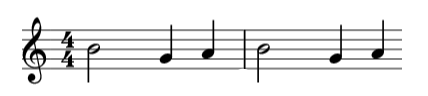
\includegraphics[scale=0.4]{obrazky-figures/rep.png}
    \caption{Obrázok opakovania taktu.}
    \label{fig:repetition}
    \end{figure}
    \item V transpozícii sa motív prenesie na ďalšiu úroveň kmitočtu. Napríklad nota h má kmitočet 494 Hz, takže na ďalšej úrovni bude mať dvojnásobný kmitočet 987 Hz. Príklad tohto posunu je na obrázku \ref{fig:transpozicia}.
    \begin{figure}[H]
    \centering
    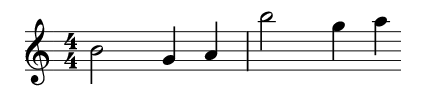
\includegraphics[scale=0.4]{obrazky-figures/trans.png}
    \caption{Obrázok transpozície taktu.}
    \label{fig:transpozicia}
    \end{figure}
    \item Postupnosť v tomto prípade znamená prenesenie motívu konštantne o jeden tón vyššie alebo o jeden tón nižšie. Na obrázku \ref{fig:Postupnost} je motív v druhom takte prenesený o jeden tón nižšie a v treťom takte je prenesený o jeden tón vyššie oproti prvému taktu.
    \begin{figure}[H]
    \centering
    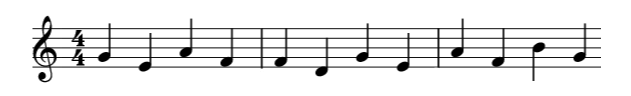
\includegraphics[scale=0.4]{obrazky-figures/Post.png}
    \caption{Obrázok postupného zvyšovania a znižovania pôvodného taktu.}
    \label{fig:Postupnost}
    \end{figure}
    \item V protipohybe sa zoberú intervaly z prvého taktu, ktorý je v tomto prípade motív. Potom v ďalšom takte sa tieto vzdialenosti tónov invertujú. V prvom takte na obrázku \ref{fig:Protipohyb} sú vzdialenosti medzi tónmi 2, -1, -2. V druhom takte sú vzdialenosti medzi tónmi -2, 1 a 2.
    \begin{figure}[H]
    \centering
    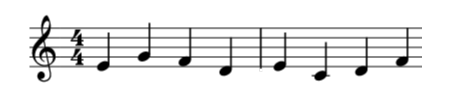
\includegraphics[scale=0.4]{obrazky-figures/Proti.png}
    \caption{Obrázok protipohybu pôvodného taktu.}
    \label{fig:Protipohyb}
    \end{figure}
    \item Retrogradácia v hudbe je zopakovanie nôt z pôvodného motívu v opačnom poradí. Napríklad, ako je motív v prvom takte na obrázku \ref{fig:Preklopenie} v poradí tónov d, g, e tak jeho variácia v druhom takte je e, g d.
    \begin{figure}[H]
    \centering
    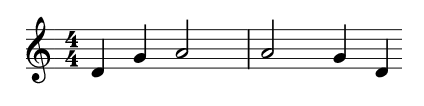
\includegraphics[scale=0.4]{obrazky-figures/Prek.png}
    \caption{Obrázok retrogradácie taktu.}
    \label{fig:Preklopenie}
    \end{figure}
    \item V prípade variovania témy predlžovaním alebo znižovaním dĺžky nôt je motív opakovaný. Variovanie motívu prebieha na obrázku \ref{fig:augmentacia} zdvojnásobením pôvodnej dĺžky noty. Keďže je stále potrebné dodržať rytmus taktu, tak sa museli posledné dve noty presunúť do extra taktu. Z taktového predpisu jeden takt môže obsahovať 4 doby. Po zdvojnásobení tejto dĺžky je potrebné rozložiť 8 dôb do dvoch taktov.
    
    Na obrázku \ref{fig:Diminution} je dvojnásobné zníženie dĺžky nôt. Keďže takt trvá 4 doby, potom jeho polovičné zníženie trvá 2 doby. Pre dodržanie tohto taktového predpisu je k dvom dobám pridaná pomlčka, ktorá trvá 2 doby. Pomlčky nie sú súčasťou práce, ale v tomto prípade sú použité pre korektný zápis taktu.    Na obrázku \ref{fig:Diminution} je dvojnásobné zníženie dĺžky nôt. Keďže takt trvá 4 doby, potom jeho polovičné zníženie trvá 2 doby. Pre dodržanie tohto taktového predpisu je k dvom dobám pridaná pomlčka, ktorá trvá 2 doby. Pomlčky nie sú súčasťou práce, ale v tomto prípade sú použité pre korektný zápis taktu.


    
    \begin{figure}[H]
    \centering
    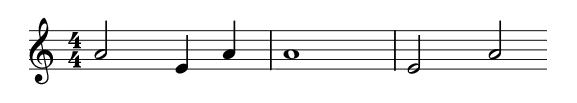
\includegraphics[scale=0.4]{obrazky-figures/Aug.png}
    \caption{Predĺženie dĺžky taktu.}
    \label{fig:augmentacia}
    \end{figure}
    \begin{figure}[H]
    \centering
    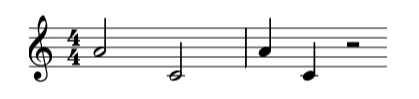
\includegraphics[scale=0.4]{obrazky-figures/Dimi.png}
    \caption{Skrátenie dĺžky taktu.}
    \label{fig:Diminution}
    \end{figure}
\end{itemize}

\section{Formálne modely}
Zavedenie formálnych modelov bolo vyžiadané čisto matematickým prístupom k jazykom. Veľká časť týchto modelov je založená na prepisujúcich systémoch. Prepisujúce systémy sa skladajú z pravidiel, ktoré opakovane menia poradie symbolov v reťazcoch. Klasifikujeme ich do dvoch základných kategórií. Generatívne modely, ktoré nazývame gramatikami definujú reťazce svojich jazykov. Tieto reťazce sú vygenerované pravidlami prepisovacieho systému z počiatočného symbolu. Prijímajúce modely, ktoré nazývame automatmi definujú reťazce svojich jazykov pomocou prepisovacieho procesu. Tento proces začína z týchto reťazcov a končí prvkom z predom danej konečnej množiny reťazcov.

\label{sec:formallang}
\subsection{Množina}
Skupinu elementov, ktoré sú prevzaté z nejakého dopredu dohodnutého prostredia nazývame množinou $\Sigma$. Element $a$ patrí množine $M$ vtedy, ak sa v nej nachádza. Zapisujeme to ako $a \in \Sigma$. V prípade, že sa v množine nenachádza zapíšeme to ako $a \not \in  \Sigma$. Ak počet prvkov v množine vieme spočítať, potom o množine hovoríme, že je konečná. Ak prvky nespočítame, potom je množina nekonečná. Konečná množina, ktorá neobsahuje žiadne prvky je prázdna množina. Prázdnu množinu označujeme ako $\emptyset$.

Konečnú množinu $\Sigma$ môžeme špecifikovať vypísaním jej elementov. Obsah množiny zapíšeme ako $\Sigma = \{a_1, a_2, a_3, ..., a_n\}$, kde prvky $a_1, a_2, a_3, ..., a_n$ patria množine $\Sigma$.

V práci s množinami využívame rôzne operácie ako sú zjednotenie, prienik a rozdiel. Zjednotenie dvoch konečných množín $\Sigma$ a $\Omega$ definujeme ako $\Sigma \cup \Omega = \{a | a \in \Sigma \: alebo  \: a \in \Omega \}$, ich prienik $\Sigma \cap \Omega = \{a | a \in \Sigma \: z\acute{a}rove\check{n}  \: a \in \Omega \}$, a rozdiel $\Sigma \setminus \Omega = \{a | a \in \Sigma \: z\acute{a}rove\check{n}  \: a \not \in \Omega \}$.

\subsection{Relácia}
Majme dva objekty $x$ a $y$. Pod označením $(x,y)$ rozumieme usporiadanú dvojicu objektov $x$,$y$ v tomto poradí. Majme dve množiny $X$ a $Y$. Kartézsky súčin $X$,$Y$ značíme ako $X \times Y$. Definujeme ho ako $X \times Y = \{(x,y) | x \in X \, a \, y \in Y\}$. Na základe týchto znalostí môžeme definovať reláciu. Reláciou $r$, ktorá je od $X$ po $Y$ rozumieme hociakú podmnožinu $X \times Y$. $r \subseteq X \times Y$ označuje nami definovanú reláciu.

\subsection{Abeceda}
Abecedou $\Sigma$ nazývame konečnú množinu, ktorá obsahuje prvky nazývané symbolmi.

\subsection{Reťazec}
Reťazcom nad abecedou $\Sigma$ nazývame konečnú postupnosť symbolov abecedy $\Sigma$. Reťazec, ktorý neobsahuje symboly sa nazýva prazdny reťazec a označujemeho ako $\varepsilon$. $\Sigma^*$ označuje množinu všetkých možných reťazcov nad abecedou $\Sigma$. $\Sigma^+$ označuje $\Sigma^* \setminus \{\varepsilon\}$. Pre $x \in \Sigma^*$ označenie $|x|$ vyjadruje počet symbolov v reťazci x. Podmnožina $L$, pre ktorú platí $L \subseteq \Sigma^*$ je formálnym jazykom nad $\Sigma$. V prípade, že $L$ je konečná množina reťazcov, potom je konečným jazykom. Naopak, ak L je nekonečná množina reťazcov, potom je nekonečným jazykom. Rodina jazykov je množina, ktorej prvky sú jazyky.

\subsection{Gramatiky}
Podsekcia gramatik má za cieľ zadefinovať gramatiky, ktoré sa vyskytujú v Chomského hierarchii. Gramatiky umožňujú vytvoriť jazyky, ktoré zapadajú do rôznych časti Chomského hierarchie. Postupným zistením, do ktorej rodiny jazykov patrí hudobný jazyk sa zameriame na jednu skupinu gramatik. Tá gramatika by vo výsledku generovala hudobné jazyky.

\begin{definition}
\label{def:frazgram}
Frázovú gramatiku definujeme ako štvoricu $G = (N,T,P,S)$, ktorá sa skladá z 
\begin{itemize}\itemsep0.05em
    \item abecedy neterminálov N
    \item abecedy terminálov T, kde platí $N \cap T = \emptyset$
    \item konečnej relácie P, ktorá je od $\{N \cup T\}^*N\{N \cup T\}^*$ po $\{N \cup T\}^*$
    \item počiatočný symbol S pre ktorý platí $S \in N$
\end{itemize}

Množina V = $N \cup T$ vyjadruje kompletnú abecedu gramatiky G. Prepisujúce pravidlá sa skladajú z dvojíc $(u,v) \in P$, ktoré označujeme ako $u \rightarrow v$. Mazacie pravidlo označujeme ako $u \rightarrow v, v = \varepsilon$. Frázové gramatiky generujú rekurzívne spočítatelné jazyky. Rekurzívne spočítatelné jazyky vedia prijať Turingové stroje.
\end{definition}

\begin{definition}
\label{def:kontextgram}
Kontextová gramatika je frázová gramatika $G = (N,T,P,S)$, ktorá sa skladá z prepisovacích pravidiel $u \rightarrow v$ vo forme $$u = x_1Ax_2, v = x_1yx_2.$$ Platí, že $A \in N$, $x_1, x_2 \in V^*$. Ďalej $y \in V^+$. Potom hovoríme o kontextovej gramatike. Kontextové gramatiky generujú kontextové jazyky. Kontextové jazyky vieme prijať linearne ohraničenými automatmi.
\end{definition}

\begin{definition}
\label{def:nonkontextgram}
Bezkontextová gramatika je frázová gramatika $G = (N,T,P,S)$, ktorá sa skladá z prepisovacích pravidiel vo forme $$A \rightarrow x.$$ Tu platí $A \in N$, $x \in V^*$. Bezkontextové gramatiky generujú bezkontextové jazyky. Bezkontextové jazyky vedia prijať zásobníkové automaty.
\end{definition}
% 87 a 246 priklady
\begin{definition}
\label{def:lingram}
Lineárna gramatika je frázová gramatika $G = (N,T,P,S)$, ktorej všetký pravidla sú v tvare $$A \rightarrow xBy, alebo \, A \rightarrow x.$$ Kde A,B $ \in N$ a x,y $ \in T^*$. Lineárny jazyk je generovaný linearnou gramatikou.
\end{definition}

\begin{definition}
Regulárna gramatika je frázová gramatika $G = (N,T,P,S)$, ktorá sa môže skladať z pravidiel vo forme $$A \rightarrow aB , alebo \, A \rightarrow a.$$ Pravidla sa skladajú z A,B $ \in N$, $a \in T$. Regulárne gramatiky generujú regulárne jazyky. Pre prijatie regulárnych jazykov používame konečné automaty.
\end{definition}

\begin{definition}
\label{def:pravolin}
Rodina regulárnych jazykov môže byť popísaná pravo-lineárnimi gramatikmi, ktoré sú definované nasledovne. Pravo-lineárna gramatika je frázova gramatika $G = (N,T,P,S)$, ktorá má všetky pravidla v tvare $$A \rightarrow aB, alebo \, A \rightarrow a.$$ Platí, že A,B $ \in N$ a x,y $ \in T^*$. Pravo-lineárny jazyk je generovaný pravo-lineárnou gramatikou.
\end{definition}

\subsection{Automaty}
Podsekcia automaty definuje základne prostriedky, ktoré sa používajú pre ropoznanie reťazcov. Tieto reťazce patria rôznym jazykom. V prípade, že daný reťazec nepatrí jazyku, ktoré prijma konkrétny automat, tak je tento reťazec odmietnuty. Ich využitie leží v prijatí hudobného jazyka.

\begin{definition}
\label{def:endaut}
Konečný automat je definovaný ako pätica $M = (Q,\Sigma,R,s,F)$, ktorá sa skladá z
\begin{itemize}\itemsep0.05em
    \item konečnej množiny stavov $Q$,
    \item vstupnej abecedy $\Sigma$,
    \item množiny pravidiel alebo prechodov $R$, ktoré sú konečnou reláciou $R \subseteq Q \times \Sigma^* \times Q$,
    \item počiatočného stavu $s \in Q$,
    \item množiny konečných stavov $F \subseteq Q$.
\end{itemize}

Pravidla sú vo forme $py \rightarrow q \in R$ na rozdiel od $(p,y,q) \in R$. Ak $y \neq \epsilon$, potom hovoríme, že $M$ je bez epsilon prechodov. Konfiguráciu automatu $M$ tvorí hociktorý reťazec z $Q \, \Sigma^*$. Značenie $\vdash_M$ značí reláciu pohybu, ktorá je definovaná ponad $Q \, \Sigma^*$ ako $$pyx \vdash_M qx.$$ Definícia platí ak a jedine ak $pyx, qx \in Q \, \Sigma^*$, a zároveň $py \rightarrow q \in R$. $L(M)$ značí jazyk automatu $M$, ktorý je  definovaný $$L(M) = \{w \in \Sigma^* \shortmid sw \vdash_M^* \, f, f \in F\}.$$
\end{definition}

\begin{definition}
\label{def:zasaut}
Zásobnikový automat je konečný automat obohatený o zásobnik. Zásobníkový automat je teda definovaný sedmicou $M = (Q,\Sigma, \Gamma , R,s,S,F)$, ktorá sa skladá z
\begin{itemize}\itemsep0.05em
    \item konečnej množiny stavov $Q$,
    \item vstupnej abecedy $\Sigma$,
    \item zásobnikovej abecedy $\Gamma$,
    \item pravidiel alebo prechodov $R$, ktoré sú konečnou reláciou $R \subseteq \Gamma^* \times Q \times (\Sigma \cup \{\epsilon\}) \times \Gamma^* \times Q$,
    \item počiatočného stavu $s \in Q$,
    \item počiatočného symbolu zásobnika $S$,
    \item množiny konečných stavov $F \subseteq Q$.
\end{itemize}
Pravidlá sú vo forme $\gamma pa \rightarrow wq$ na rozdiel od $(\gamma , p, a, w, q) \in R$. Konfiguráciu automatu $M$ tvorí hociktorý reťazec z $\Gamma^* Q\Sigma^*$. Značenie $\vdash_M$ značí reláciu pohybu, ktorá je definovaná ponad $\Gamma^* Q\Sigma^*$ ako $$x\gamma pay \vdash_M xwqy.$$ Definícia platí ak a jedine ak $x\gamma pay, xwqy \in \Gamma^* Q\Sigma^*$, a zároveň $\gamma pa \rightarrow wq \in R$. Existujú rôzne spôsoby ako prijať jazyk zásobníkovým automatom. Súvisiaci je ale jeden spôsob, a to s prázdnym zásobníkom. $L_e(M)$ značí jazyk automatu $M$, ktorý prijíma jazyk prázdnym zásobníkom nasledovne $$L_e(M) = \{w \in \Sigma^* \shortmid Ssw \vdash_M^* \,q,q \in Q\}.$$
\end{definition}

\subsection{Chomského hierarchia}
Frázové, kontextové, bezkontextové a regulárne gramatiky tvoria jazyky typ-0, typ-1, typ-2 a typ-3. Rodina jazykov generovaná pravo-linárnimi gramatikami sú si rovné s rodinou jazykov, ktoré sú generované regulárnymi gramatikami. Preto označenia RVJ, KJ, BJ, LINJ, REJ sú použité pre rodiny jazykov generovaných všeobecnými, kontextovými, bezkontextovými, lineárnymi a regulárnymi gramatikami. RLINJ je označenie pre rodinu jazykov generovanú pravo-lineárnymi gramatikami. Pre tieto rodiny jazykov platí inklúzia $REJ = PLINJ \subset LINJ \subset BJ \subset KJ \subset RVJ$. Popis tejto hierarchie a jej prepojenie s hudbou je prevzaté z \cite{jstorgrammusic, musicformallang}.

\begin{figure}[H]
    \centering
    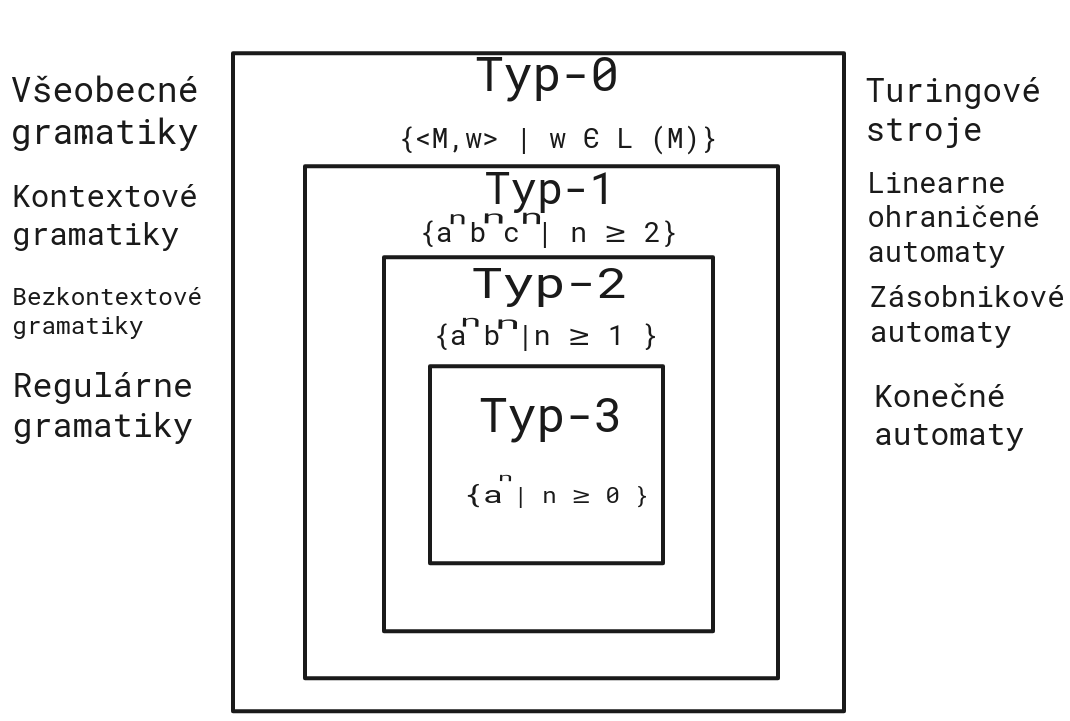
\includegraphics[scale=0.3]{obrazky-figures/ChomHier.png}
    \caption{Chomského hierarchia slabej generativnej kapacity.}
    \label{fig:chomhier}
\end{figure}

Obrázok sme prevzali z \cite{musicformallang}.

\subsection*{Typ-3 (Regulárne jazyky)}
Regulárne jazyky sa používajú napríklad pre zápis regulárnych výrazov. Tie sa využívajú v rôznych UNIX-ových nástrojoch. Tieto jazyky sú výpočtovo nenáročné, deterministicky spracovateľné v lineárnom čase a podporujú rôzne matematické operácie, ako sú napríklad zjednotenie alebo konkatenacia. Ich najväčšia nevýhoda oproti silnejším formálnym modelom je ich limitovaná generatívna kapacita.

Regulárne gramatiky sú taktiež veľmi limitujúce v tom, že nedokážu vytvoriť viacúrovňovú stromovú štruktúru, ktorou hudobná štruktúra určite je. Je to kvôli obmedzeniu gramatiky, u ktorej musí byť jeden neterminal na pravej strane produkčných pravidiel. Spracovanie hudobnej štruktúry si vyžaduje minimálne možnosť spracovať vnorené závislosti, ktoré sa v hudbe vyskytujú. Túto možnosť regulárne gramatiky neponúkajú. Príkladom stromovej štruktúry môže byť variácia na obrázku \ref{fig:Preklopenie}.

Spočiatku sa ponúkala ako vhodné riešenie pravo-lineárna gramatika definovaná v \ref{def:pravolin}. Tieto gramatiky spadajú na základe Chomského hierarchie do tejto kategórie. Pravidlami tejto gramatiky by sme mohli popísať tvorbu jednotlivých tónov. Majme pravidlo pravo-lineárnej gramatiky $A \rightarrow aB$. Ak vieme dosadiť za $a$ nejaký tón, potom vieme deriváciami tvoriť reťazce tónov tvoriace hudbu. Napriek tomu, že ponúkajú túto možnosť, nie je ich možné použiť pre popis hudobnej štruktúry alebo tvorby hudobných pasáži. Variácie, ktoré sú rozoberané vyššie maju medzi sebou rôzne križiace a vnorené závislosti. Tieto vlastnosti pripisujeme jazykom typ-2 a typ-1 a nie je možné ich popísať regulárnymi a pravo-lineárnymi gramatikami. Uplatnenie týchto gramatik by bolo možné v prípade využitia derivácií pre tvorenie hudby. Samozrejme, že derivačné kroky by museli byť riadené nejakým spôsobom. Jedným z nich by bola náhodnosť. Pri taktomto postupe nie je možné zaručiť rozumný výsledok. Výsledok takéhoto postupu by nemusel byť vhodný na počúvanie, pretože by sa skladal z náhodného zhluku tónov.

Markovské procesy, ktoré boli charakterizované Chomskym patria medzi typu-3 a nepreukázali schopnosť spracovať frázovú štruktúru. Tieto limitácie nesúvisia s problematikou stochastických procesov a deterministickych procesov. Limitácie sa týkajú produkčných pravidiel. Markovské procesy sa riadia lineárnymi krokovými pravidlami narozdiel od bezkontextových gramatík. Bezkontextové gramatiky umožňujú vytvoriť reťazec neterminálov naraz, pomocou produkčných pravidiel. Na základe týchto skutočností vieme, že regulárne gramatiky neponúkajú vhodne riešenie k popisu hudobnej štruktúry.

\subsection*{Typ-2 (Bezkontextové jazyky)}
Tieto jazyky sa vyznačujú štruktúrami, ktoré sú reprezentované balancovanými stromami a ďalšími zrkadliacimi sa štruktúrami. Obrovské využitie týchto jazykov je u programovacích jazykoch, ktoré sú ich deterministický spracovateľnou podmnožinou. Jazyky typu-2 prinášajú so sebou nejednoznačnosť a neplatia u nich operácie doplnok, prienik a ďalšie. Tieto jazyky sú spracovateľné v $O(n^3)$ čase.

Určité časti hudobnej štruktúry, ktoré sú reprezentované hudobnými reťazcami vieme zaradiť medzi bezkontextové jazyky. Ide o motív alebo tému, ktorá postupne rastie a následne rovnakými tonami klesá. Tento jav tvorí zrkadlovú štruktúru, ktorá je zobrazená na ľavej strane obrázku \ref{fig:dependencies}.

Tieto gramatiky sú jednoduchšie na spracovanie oproti gramatikám, ktoré tvoria jazyky v nadchádzajúcich sekciách. Je to vďaka tomu, že umožňujú reťazce iba na jednej strane produkčných pravidiel. Zložitosť je teda lineárna k počtu neterminálov v derivácií. Sila bezkotextových gramatik leží v tom, že umožňujú reprezentáciu viacúrovňových vnorených syntaktických štruktúr. Neterminal, ktorý môže reprezentovať motív, frázu, vetu alebo sekciu generuje reťazec tokenov na nižšej úrovni. Schopnosť generovať reťazce tokenov v jednom z produkčných pravidiel, ich robí lepším kandidátom k popisu hudobnej štruktúry, narozdiel od regulárnych gramatík.

\begin{figure}[H]
    \centering
    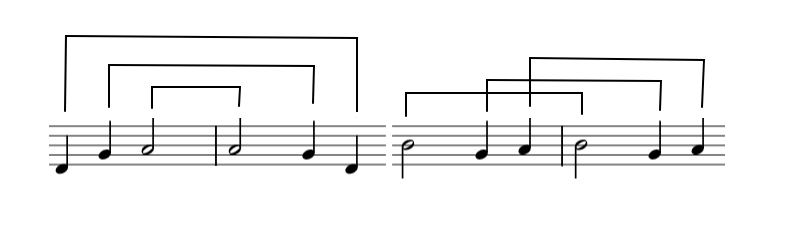
\includegraphics[scale=0.4]{obrazky-figures/zavislosti.png}
    \caption{Znázornenie vnorených a kopírujúcich sa závislosti na variáciach.}
    \label{fig:dependencies}
\end{figure}

V tejto kategórii sa nachádzajú jazyky tvorené gramatikami \ref{def:nonkontextgram} a \ref{def:pravolin}. Tieto gramatiky stačia pre popis len niektorých části hudobných pasáži, ktoré sa vyskytujú len v určitých častiach hudby. Jednou štruktúrovanou časťou sú variácie základnej témy retrogradáciou, ktorú môžeme vidieť na obrázku \ref{fig:Preklopenie}. Druhou časťou sú úseky hudby, ktoré nie sú štruktúrované do témy a jej variácie. Napriek tomu, že nie sú štruktúrované do témy a variácií tvoria reťazce, ktoré sú bezkontextové. Príkladom v hudbe môžu byť rôzne vsuvky, medzihry alebo vyhrávky. Tieto hudobné pasáže majú melodický a ozdobný charakter, ktoré sú charakterizovateľné vnorenými závislosťami bezkontextových jazykov.

\subsection*{Typ-1 (Kontextové jazyky)}
Kontextové jazyky zahrňujú v sebe aj kopírovacie jazyky. Tieto jazyky sú rozhodnutelné, ale vyžadujú si vysokú výpočtovú silu vo väčšine prípadov. Ukázalo sa, že v niektorých prípadoch hudobné reťazce si vyžadujú silnejší formalizmus, ako sú bezkontextové gramatiky. Je to vďaka tomu, že tóny sú medzi jednotlivými taktami usporiadané vo forme kopírovacích jazykov. Ukážka takéhoto jazyka v notovom zápise je na pravej strane obrázka \ref{fig:dependencies}. Zápis tohto jazyka by mohol vyzerať ako $h^ng^na^n$. Vo väčšine prípadov bude n nastavené na 2. Viac opakovaní nie je úplne zmysluplné, pokiaľ nechceme aby zneli tieto dva takty točili v slučke.

S kontextovými gramatikami prichádzajú aj problémy. Prvý problém je, že reťazce vygenerovane touto gramatikou sú nerozhodnutelné. Nerozhodné pravidlá sú súčasťou tejto gramatiky, čo znemožňuje zachovanie rovnakej frázovej štruktúry v reťazcoch generovaných kontextovou gramatikou. To je spôsobené tým, že každá strana z produkčných pravidiel môže byť reťazec tokenov. Reťazce tokenov na každej strane znemožňujú aplikáciu kontextových gramatik v analýze hudobnej štruktúry. Bezkontextové gramatiky môžu mať tiež nerozhodné pravidlá, ale krokovanie ich derivácií je zjednodušené. Zjednodušením je hociaký terminál, ktorý sa redukuje na jediný neterminal narozdiel od kontextových gramatik. U kontextových gramatík sa môže redukovať na celý reťazec.

Druhým problémom je implementácia. Použitie prekladača na takúto gramatiku spôsobuje znásobenie počtu produkčných pravidiel počtom kontextových možnosti. Špecifikácia takejto gramatiky nie je jednoducha. Popisovanie krokov gramatiky takého prekladača sa stane kombinatorické, pretože krížové závislosti musia byť vložené do produkčných tabuliek.

Napriek všetkým týmto komplikáciám je stále možné kontextové závislosti zabudovať do gramatiky konštruovanej čisto z bezkontextových produkčných pravidiel. Tento spôsob je možné celkom jednoznačne preložiť. Problem môže nastať u zobrazovaní kopírovacích závislostiach v gramatike.

Gramatika \ref{def:kontextgram} generujúca jazyky, ktoré patria medzi kontextové sa ukázala ako vhodný kandidát pre popis hudobnej štruktúry. Vďaka tomu, že na oboch stranách pravidiel vieme dosadiť reťazce, potom sa dá jednoducho popísať notový zápis na pravej strane na obrázku \ref{fig:dependencies}. Deriváciami kontextovej gramatiky vieme pokryť tvorbu všetkých variácií. Nedeterministickosť kontextových gramatík neobmedzuje tvorby takej štruktúry, ako je téma~a jej variácie. Práve naopak je táto vlastnosť vítaná, pretože nezväzuje ruky tvorcovi tejto štruktúry. Táto gramatika bude musieť umožniť tvorbu každej križiacej sa závislosti, ktoré obsahujú variácie. Konkrétna gramatika, ktorá bola použitá pre popis tejto štruktúry bude rozoberaná v nasledujúcej kapitole.

\subsection*{Typ-0 (Rekurzívne spočítatelné jazyky)}
Rekurzívne spočítatelné jazyky sú jazyky, ktoré sú tvorené všeobecnými gramatikami. Tieto gramatiky nezavádzajú žiadne obmedzenia na produkčné pravidla. Z definície tieto gramatiky umožňujú vznik nekonečných reťazcov, ktoré samotné v hudbe nepredstavujú zmysel a nevedú tak k rozumnému riešeniu. Existujú ale hudobné prostredia, ktoré sa zaoberajú generovaním a syntézou v reálnom čase. Tieto prostredia sú turingovo úplne a volia si silnú generatívnu kapacitu. Problém s výpočtovou náročnosťou nechávajú v rukách užívateľa. Definícia \ref{def:frazgram} definuje gramatiku, ktorá generuje tieto jazyky. Využitie tejto gramatiky nie je momentálne v tejto práci, ale využitie môžu nájsť v jej ďalšom vývoji tejto práce.

\chapter{Návrh modelu pre tvorbu nových hudobných pasáži}
\label{chap:app}
Obsahom tejto sekcie je návrh nových verzii modelov, ktoré by sa mohli aplikovať v hudbe. Návrh vychádza z gramatík s rozptýleným kontextom, ktoré sa ukázali vhodné v mnohých aspektoch tvorby hudby. Ako obrovská výhoda sa ukázala preskočenie kontextu, ktorý sa v rôznych pasážiach hudby vyskytuje. Ich ďalšou výhodou je, že umožňujú generovanie bezkontextových jazykov, ale i kontextových jazykov. Gramatiky s rozptýleným kontextom našli aplikácie v lingvistike. Aplikácia týchto gramatik v lingvistike je podobného princípu, ako sú aplikácie v hudbe. Na základe toho sa ukázali gramatiky s rozptýleným kontextom vhodné pre aplikáciu v hudbe. Teória ku gramatikam s rozptýleným kontextom a ich aplikáciam je prevzatá z knižiek \cite{FITPUB8997, FITPUB10498}.

\section{Gramatika s rozptýleným kontextom}
\begin{definition}
Gramatikou s rozptýleným kontextom rozumieme štvoricu \\ $G = (V,T,P,S),$ ktorá sa skladá z
\begin{itemize}\itemsep0.05em
    \item úplnej abecedy V 
    \item množiny terminálov T, pre ktorú platí $T \subset V$
    \item konečnej množiny pravidiel P v tvare $$(A_1, ..., A_n) \rightarrow (x_1, ..., x_n),$$ kde platí $n \geq 1, A_i \in V \setminus T, x_i \in V^*$ pre všetky i $1 \leq i \leq n.$
    \item počiatočného symbolu S pre ktorý platí $S \in V \setminus T$
\end{itemize}
\end{definition}

V prípade, že $$u = u_1A_1...u_nA_nu_{n+1},$$$$v = u_1x_1...u_nx_nu_{n+1},$$ ako aj $p = (A_1, ..., A_n) \rightarrow (x_1, ..., x_n) \in P,$ kde $u_i \in V^*$, pre každé i ohraničené podmienkou $1 \leq i \leq n + 1$, máme derivačný krok od $u$ po $v$ na základe $p$ vytvorený gramatikou $G$, ktorý zapisujeme $u \Rightarrow_G v \, [p],$ alebo zjednodušenou variantou $u \Rightarrow_G v$.

Ak platí $dl\check{z}ka(p) \geq 2$, potom hovoríme, že $p$ je kontextovým pravidlom. V prípade, že $dl\check{z}ka(p) = 1$ tak $p$ je bezkontextové pravidlo. Jazyk značený ako $L(G)$ je generovaný gramatikou $G$ a definujeme ho ako $$L(G) = \{x: x \in T^*, S \Rightarrow^*_G x\}.$$

Jazyk s rozptýleným kontextom je jazyk $L$ práve vtedy, ak vieme nájsť takú gramatiku s rozptýleným kontextom $G$, kedy platí $L = L(G)$. Gramatiky s rozptýleným kontextom generujú jazyky s rozptýleným kontextom, ktoré označujeme ako $JRC$.

\begin{example}
    Zoberme si jazyk typu-1, ktorý je zobrazený na obrázku \ref{fig:chomhier} \\ $L = \{a^n b^n c^n| n \geq 2\}$. Aby sme mohli tento jazyk generovať gramatikou v hudbe je potrebné ho zapísať pomocou tónov. Tento jazyk vyzerá nasledovne: $L = \{c^n d^n e^n| n \geq 2\}$. Aby sme vygenerovali tento jazyk pomocou gramatiky s rozptýleným kontextom definujeme ju nasledovne: $$ G = (\{S, X, c, d, e\}, \{c,d,e\}, P, S)$$ kde $$P = \{(S) \rightarrow (ccXddXeeX), (X,X,X) \rightarrow (cX, dX, eX), (X,X,X) \rightarrow (\epsilon, \epsilon, \epsilon)\}.$$
    Majme užívateľa, ktorý by chcel vytvoriť hudobnú myšlienku v tvare $cccdddeee$. Myšlienka by bola vytvorená nasledovne: $$ S \Rightarrow_G  ccXddXeeX \Rightarrow_G cccXdddXeeeX \Rightarrow_G cccdddeee.$$
\end{example}

Samotná gramatika s rozptýleným kontextom sa ukázala ako vhodná pre generovanie rôznych hudobných jazykov. Pod týmito jazykmi rozumieme $JRC$. Tento prístup je vhodný v prípade, že užívateľ vie ako by mal výstup vyzerať. No v prípade hudobníkov to vždy tak nie je. Predstavme si hudobníka, ktorý si nosí v hlave nejakú tému skladby. Dopredu nevie povedať ako bude vyzerať variácia tejto hudobnej myšlienky. Variácie existujú rôzne a vybrať si jednu, ktorá by sa mu hodila pre pokračovanie ďalej v skladbe vôbec nie je jednoduché. Zložitosť predstaviť si takú variáciu narastá s dĺžkou témy, od ktorej by sa mala rozvíjať. Princíp tohto riešenia môžeme spozorovať na pravej strane obrázku \ref{fig:dependencies}. Kedy by sa mohla v prvom takte nachádzať nejaká myšlienka skladateľa, a na druhej strane jej obmenenie, čiže variácia. Hovoríme teda o spomínanom kopírovacom jazyku, a krížiacich sa závislostiach. Krížiace sa závislosti je možné reprezentovať gramatikami s rozptýleným kontextom. Príklad gramatiky, ktorá vytvorí reťazec z obrázka je nasledovný.

\begin{example}
\label{variation}
Reťazec tónov z obrázka \ref{fig:dependencies} sa skladá v dvoch taktoch z tónov $hgahga$. Majme gramatiku $$G = (\{S,X,h,g,a\}, \{h,g,a\}, P, S)$$ kde $$P = \{(S) \rightarrow (XX), (X,X) \rightarrow (hX,hX)$$ $$(X,X) \rightarrow (aX,aX), (X,X) \rightarrow (gX,gX), (X,X) \rightarrow (\epsilon, \epsilon)\}.$$ Postup tvorby spomínaných dvoch taktov je nasledovný: $$S \Rightarrow_G XX \Rightarrow_G hXhX \Rightarrow_G hgXhgX \Rightarrow_G hgaXhgaX \Rightarrow_G hgahga.$$
\end{example}

Na príklade \ref{variation} môžeme spozorovať, že gramatika generuje jazyk, ktorý nie je bezkontextový. Tento jazyk je $JRC$. Vytvorený reťazec demonštruje, že týmto spôsobom vieme vytvoriť požadovanú štruktúru téma a variácie.

Môžeme si všimnúť, že stále zanedbávame dĺžky jednotlivých tónov. Riešenie bude prezentované v nadchádzajúcej kapitole.

\section{Spracovanie nôt}
V tejto sekcii si rozoberieme akým spôsobom sú ďalej reprezentované noty. Reprezentácia nôt v programe nie je vôbec jednoduchá. Sú to grafické značky a zapisujú sa do notového zápisu, ktorý je tiež grafický. Toto znemožňuje ich jednoduchú reprezentáciu ako v programe, ale i vo vstupnom súbore. Keď sa pozrieme do notového zápisu nejakého taktu tak vidíme samotnú značku. Ako prvé podľa jej tvaru vieme odčítať jej dĺžku či ide o celú, polovú, štvrťovú alebo osminovú notu. Ak chceme zistiť tón tak ho odčítame z pozície noty v notovej osnove. Preto boli zavedené nasledovné značenia pre jednotlivé noty.

\begin{table}[!ht]
\label{tab:tone}
    \centering
    \begin{tabular}{|l|l|l|l|l|l|l|l|l|l|l|l}
    \hline
        ~ & c1 & d1 & e1 & f1 & g1 & a1 & h1 \\ \hline
        celá & c1\_c & d1\_c & e1\_c & f1\_c & g1\_c & a1\_c & h1\_c \\ \hline
        polová & c1\_p & d1\_p & d1\_p & f1\_p & g1\_p & a1\_p & h1\_p \\ \hline
        štvrťová & c1\_š & d1\_š & d1\_š & f1\_š & g1\_š & a1\_š & h1\_š \\ \hline
        osminová & c1\_o & d1\_o & d1\_o & f1\_o & g1\_o & a1\_o & h1\_o  \\ \hline
    \end{tabular}
    \caption{\label{tab:notes} Prehlad popisu nôt.}
\end{table}
\begin{table}[!ht]
    \centering
    \begin{tabular}{|l|l|l|l|l|l|l|l|l|l|l|l}
    \hline
        ~ & c2 & d2 & e2 & f2 & g2 & a2 & h2 & c3 \\ \hline
        celá & c2\_c & d2\_c & e2\_c & f2\_c & g2\_c & a2\_c & h2\_c & c3\_c \\ \hline
        polová & c2\_p & d2\_p & e2\_p & f2\_p & g2\_p & a2\_p & h2\_p & c3\_p \\ \hline
        štvrťová & c2\_š & d2\_š & e2\_š & f2\_š & g2\_š & a2\_š & h2\_š & c3\_š \\ \hline
        osminová & c2\_o & d2\_o & e2\_o & f2\_o & g2\_o & a2\_o & h2\_o & c3\_o \\ \hline
    \end{tabular}
    \caption{\label{tab:notes1} Prehlad popisu nôt.}
\end{table}

Tabuľky \ref{tab:notes} a \ref{tab:notes1} zobrazujú ako boli pomenované jednotlivé terminály, ktoré sú použité ďalej v práci. Stĺpce tabuľky sú pomenované po tónoch, ktoré sa nachádzajú na jednočiarkovanej a dvojčiarkovanej oktáve. Existuje množstvo tónov, ale tieto sú v bežných skladbách najpoužívanejšie. Riadky tabuľky sú pomenované po jednotlivých dĺžkach tónov, ktoré sú použité v tejto práci.

\section{LL gramatika s rozptýleným kontextom}
Táto sekcia sa zaoberá a definuje gramatiku s lineárnymi pravidlami. Ide o $LL(k)$ verziu gramatiky s rozptýleným kontextom. Pre získanie tejto gramatiky je potrebné modifikovať gramatiku s rozptýleným kontextom. Nižšie je rozoberaný spôsob v troch bodoch, ktorý popisuje tento proces. Obsahuje aj úpravy pre potrebu tvorby hudobných pasáži, ako sú variacie. Text, ale i definície v tejto kapitole sú prevzaté z \cite{FITPUB10498}.

\begin{enumerate}[label=\arabic*)]
    \item Každé pravidlo gramatiky, ktoré by malo tvoriť hudobné pasáže sa musí skladať iba z lineárnych pravidiel. Pod tým rozumieme, že každé $x_i$ môže obsahovať naraz iba jeden neterminál. Existuje ale jedna výnimka pre pravidlo pre počiatočný symbol S v tvare $(S) \rightarrow (x)$. Pod $x$ rozumieme neprázdny reťazec, kde môže byť naraz $k$ neterminalov. Kde $k$ je pozitívne celé číslo pre každú gramatiku. Pre pravidlá ďalej platí, že $S$ sa nesmie objaviť na pravej strane.
    
    \item Majme pravidlo typu $(X,X) \rightarrow (c1\_c, c1\_c)$, ktoré vieme použiť pri kopírovaní tónov. Ak zoberieme prvé komponenty všetkých takýchto pravidiel vo forme $X \rightarrow c1\_c$, potom získame bezkontextovu gramatiku, ktorá je LL gramatikou. Viac o LL gramatikách pozri \cite{FITPUB10524}.
    
    \item Zoberme si variáciu opakovaním témy z obrázku \ref{fig:repetition}. Aby sme prepísali terminály reprezentujúce tieto tóny $HGAHGA$, potrebujeme pravidlá aplikovať iba najľavejším spôsobom. Prepísanie pravidlom $(X,X,X) \rightarrow (h1\_c, g1\_\check{s}, a1\_\check{s})$ je možné iba na $h1\_c \, g1\_\check{s} \, a1\_\check{s}HGA$. Teda $HHGGAA$ nie je možné prepísať týmto spôsobom. To nie je potrebné, pretože tieto neterminály nestvárňujú štruktúru téma a variácie.
\end{enumerate}

Pred definovaním samotnej gramatiky je potrebné definovať dva pojmy.

\begin{definition}
Majme bezkontextovu gramatiku $G = (N, T, P, S)$. Potom pre každé $x \in (N \cup T)^*$ máme množinu $$prv\acute{y}(G,x) = \{a \in T \: | \: x \Rightarrow^*_G ay \: vo \: G, y \in (N \cup T)^*\}.$$ 
\end{definition}

\begin{definition}
Majme gramatiku s rozptýleným kontextom $G = (N, T, P, S)$. Značenie $pjadro(G)$ značí prvý komponent jadra gramatiky $G$. Definujeme ho ako bezkontextovu gramatiku $$pjadro(G) = (N,T,P^\prime,S),$$ kde $$P^\prime = \{A_1 \rightarrow x_1 \, | \, (A_1, A_2, ..., A_m) \rightarrow (x_1, x_2, ..., x_m) \in P^\prime\}.$$
\end{definition}

\begin{definition}
\label{def:ll}
Majme gramatiku s rozptýleným kontextom $G = (N, T, P, S)$. Nech $k$ je kladné celé číslo. Potom hovoríme o $G$ ako o LL k-lineárnej gramatike s rozptýleným kontextom ak sú splnené tieto tri podmienky. 
\end{definition}

\begin{enumerate}[label=\arabic*)]
    \item Podmienka k-linearity. Pre každé pravidlo $P$ platí, že je vo forme $$(S) \rightarrow (x),$$ kde platí $x \in (N \setminus \{S\})^+, |x| \leq k,$ alebo $$(A_1,A_2, ..., A_m) \rightarrow (x_1, x_2, ..., x_m).$$ V pravidlách tohto typu platí, že $A_i \in (N \setminus \{S\}), x_i \in T^*(N \setminus \{S\})T^* \cup T^+,$ pre všetký i ohraničené $1 \leq i \leq m, $ pre nejaké $m \geq 1.$
    
    \item Prvá LL podmienka. Majme relaciu $\Rightarrow_G$, ktorá je definovaná derivačným krokom od u po v, značená ako $u \Rightarrow_G v$. Vtedy a iba vtedy ak $$u = u_1A_1u_2A_2...u_mA_my$$ $$v = u_1x_1u_2x_2...u_mx_my,$$ a $$(A_1,A_2, ...,A_m) \rightarrow (x_1,x_2, ..., x_m) \in P.$$ kde $y \in V^*, u_i \in T^*,$ pre všetky i, ktoré sú ohraničené $1 \leq i \leq m.$ 
    
    \item Druhá LL podmienka. Majme dve rozdielne pravidlá $$(A_1,A_2, ...,A_m) \rightarrow (x_1, x_2, ..., x_m) \in P$$ a $$(B_1, B_2, ..., B_n) \rightarrow (y_1, y_2, ..., y_n),$$ ktoré spĺňajú podmienku $A_1 = B_1$, platí že $$prv\acute{y}(pjadro(G),x_1) \cap prv\acute{y}(pjadro(G),y_1) = \emptyset$$
\end{enumerate}

\begin{example}
Majme LL 2-lineárnu gramatiku s rozptýleným kontextom \\ $G = (\{S,X\},\{c1\_p, d1\_p, |\}, P, S)$, kde $$P = \{(S) \rightarrow (XX), (X,X) \rightarrow (c1\_pX, c1\_pX), $$
$$ (X,X) \rightarrow (d1\_pX, d1\_pX, (X,X) \rightarrow (|, |)\}.$$ potom tvorba nasledujúcej dvojice taktov z obrázku \ref{fig:Priklad1} vyzerá nasledovne:
\begin{figure}[H]
    \centering
    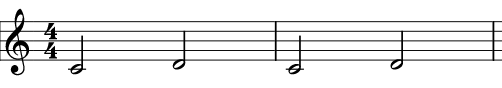
\includegraphics[scale=0.4]{thesis/obrazky-figures/Priklad1.png}
    \caption{Variácia opakovaním.}
    \label{fig:Priklad1}
\end{figure}
$$S \Rightarrow_G XX \Rightarrow_G c1\_pXc1\_pX \Rightarrow_G c1\_pd1\_pXc1\_pd1\_pX \Rightarrow_G c1\_pd1\_p|c1\_pd1\_p|.$$

Zjavne platí, že $|XX| = 2$, na pravej strane pravidiel na nevyskytuje S.
\end{example}

Aby bolo možné správne reprezentovať tvorbu variácií pomocou gramatiky, budeme musieť vytvoriť novú gramatiku, ktorá bude obsahovať určité úpravy. Preto gramatika pre tvorbu variácií je nasledovná:

\begin{definition}
\label{mainalg}
$G = (\{S, X, R, c1\_c, d1\_c, e1\_c, f1\_c, g1\_c, a1\_c, h1\_c, c2\_c, d2\_c, \\ e2\_c, f2\_c, g2\_c, a2\_c, h2\_c, c3\_c, c1\_p, d1\_p, d1\_p, f1\_p, g1\_p, a1\_p, h1\_p, c2\_p, \\ d2\_p, e2\_p, f2\_p, g2\_p, a2\_p, h2\_p, c3\_p, c1\_\check{s}, d1\_\check{s}, d1\_\check{s}, f1\_\check{s}, g1\_\check{s}, a1\_\check{s}, h1\_\check{s}, \\ c2\_\check{s}, d2\_\check{s}, e2\_\check{s}, f2\_\check{s}, g2\_\check{s}, a2\_\check{s}, h2\_\check{s}, c3\_\check{s}, c1\_o, d1\_o, d1\_o, f1\_o, g1\_o, a1\_o, \\ h1\_o, c2\_o, d2\_o, e2\_o, f2\_o, g2\_o, a2\_o, h2\_o, c3\_o, |\}, \{c1\_c, d1\_c, e1\_c, f1\_c, g1\_c, \\ a1\_c, h1\_c, c2\_c, d2\_c, e2\_c, f2\_c, g2\_c, a2\_c, h2\_c, c3\_c, c1\_p, d1\_p, d1\_p, f1\_p, \\ g1\_p, a1\_p, h1\_p, c2\_p, d2\_p, e2\_p, f2\_p, g2\_p, a2\_p, h2\_p, c3\_p, c1\_\check{s}, d1\_\check{s}, d1\_\check{s}, \\ f1\_\check{s}, g1\_\check{s}, a1\_\check{s}, h1\_\check{s}, c2\_\check{s}, d2\_\check{s}, e2\_\check{s}, f2\_\check{s}, g2\_\check{s}, a2\_\check{s}, h2\_\check{s}, c3\_\check{s}, c1\_o, d1\_o, \\ d1\_o, f1\_o, g1\_o, a1\_o, h1\_o, c2\_o, d2\_o, e2\_o, f2\_o, g2\_o, a2\_o, h2\_o, c3\_o, |\}, P, S),$ \\
kde $$P = \{\{(S) \rightarrow (XX)\} \, \cup $$
%opakovanie
$$\{(X,X) \rightarrow (c1\_cX, c1\_cX), (X,X) \rightarrow (d1\_cX, d1\_cX)$$
$$\vdots$$
$$(X,X) \rightarrow (c1\_pX, c1\_pX), (X,X) \rightarrow (d1\_pX, d1\_pX)$$
$$\vdots$$
$$(X,X) \rightarrow (c1\_\check{s}X, c1\_\check{s}X), (X,X) \rightarrow (d1\_\check{s}X, d1\_\check{s}X)$$
$$\vdots$$
%zvysenie tonov
$$\}\, \cup$$
$$\{(X,X) \rightarrow (c1\_cX, d1\_cX), (X,X) \rightarrow (d1\_cX, e1\_cX)$$
$$\vdots$$
$$(X,X) \rightarrow (c1\_pX, d1\_pX), (X,X) \rightarrow (d1\_pX, e1\_pX)$$
$$\vdots$$
$$(X,X) \rightarrow (c1\_\check{s}X, d1\_\check{s}X), (X,X) \rightarrow (d1\_\check{s}X, e1\_\check{s}X)$$
$$\vdots$$
$$\}\, \cup$$
%znizenie tonov
$$\{(X,X) \rightarrow (d1\_cX, c1\_cX), (X,X) \rightarrow (e1\_cX, d1\_cX)$$
$$\vdots$$
$$(X,X) \rightarrow (g1\_oX, f1\_oX), (X,X) \rightarrow (a1\_oX, g1\_oX)$$
$$(X,X) \rightarrow (h1\_oX, a1\_oX), (X,X) \rightarrow (c2\_oX, h1\_oX)$$
$$\vdots$$
$$\}\, \cup$$
%predlzenie
$$\{(X,X) \rightarrow (c1\_pX, c1\_cX), (X,X) \rightarrow (e1\_pX, e1\_cX)$$
$$\vdots$$
$$(X,X) \rightarrow (g1\_oX, g1\_\check{s}X), (X,X) \rightarrow (a1\_oX, a1\_\check{s}X)$$
$$(X,X) \rightarrow (h1\_oX, h1\_\check{s}X), (X,X) \rightarrow (c2\_oX, c2\_\check{s}X)$$
$$\vdots$$
$$\}\, \cup$$
%skratenie
$$\{(X,X) \rightarrow (c1\_cX, c1\_pX), (X,X) \rightarrow (e1\_cX, e1\_pX)$$
$$\vdots$$
$$(X,X) \rightarrow (g1\_\check{s}X, g1\_oX), (X,X) \rightarrow (a1\_\check{s}X, a1\_oX)$$
$$(X,X) \rightarrow (h1\_\check{s}X, h1\_oX), (X,X) \rightarrow (c2\_\check{s}X, c2\_oX)$$
$$\vdots$$
$$\}\, \cup$$
%transpozicia
$$\{(X,X) \rightarrow (c1\_cX, c2\_pX), (X,X) \rightarrow (d1\_cX, d2\_cX)$$
$$\vdots$$
$$\}\, \cup$$
%protipohyb
$$\{$$
$$\vdots$$
$$(X,X) \rightarrow (c2\_oX, d1\_oX), (X,X) \rightarrow (f1\_oX, a1\_oX)$$
$$(X,X) \rightarrow (c2\_cX, d1\_cX)$$
$$\vdots$$
$$(X,X) \rightarrow (|, |)\}\, \cup$$
$$\{(S) \rightarrow R$$
$$\vdots$$
$$R \rightarrow g1\_\check{s}Rg1\_\check{s}, R \rightarrow a1\_\check{s}Ra1\_\check{s}$$
$$R \rightarrow h1\_\check{s}Rh1\_\check{s}, R \rightarrow c2\_\check{s}Rc2\_\check{s}$$
$$\vdots$$
$$R \rightarrow |\}$$

U výslednej gramatiky platí $|XX| = 2$. Na žiadnych z pravidiel sa na pravej strane nevyskytuje počiatočný symbol S. U tejto gramatiky si môžeme všimnúť, že je porušená druhá LL podmienka z definície \ref{def:ll}. Zoberme si pravidlá $$(X,X) \rightarrow (c1\_cX, c1\_cX), (X,X) \rightarrow (c1\_cX, d1\_cX).$$ Prvé pravidlo patrí variácií kopírovaním a druhé pravidlo patrí variácií, ktorá postupne zvyšuje tému o jeden tón. Potom $$prv\acute{y}(pjadro(G),c1\_cX) \cap prv\acute{y}(pjadro(G),c1\_cX) \neq \emptyset.$$ Porušenie tejto podmienky spôsobuje nejednoznačnosť pravidiel, z ktorých je konštruovaná výsledná LL tabuľka. Riešením tohto problému je, že jednotlivé skupiny pravidiel patria príslušným variáciám. Užívateľ, ktorý si zvolí tvorbu variácie opakovaním by zvolil prvé uvedené pravidlo. Zvolenie variácie pre postupne zvýšenie témy o jeden tón vyberie druhé pravidlo. Vďaka voľbe užívateľa nedochádza k takýmto konfliktom.
\end{definition}

Definovaná gramatika obsahuje terminály, ktoré boli uvedené v tabuľkách \ref{tab:notes} a \ref{tab:notes1}. Kompletný zoznam pravidiel, ktoré boli použité v tejto práci je možné nájsť v prílohe. Vybrané pravidlá, ktoré sú uvedené vyššie boli použité na nasledujúce hudobné pasáže.

\begin{example}
Majme variáciu opakovaním.
\begin{figure}[H]
    \centering
    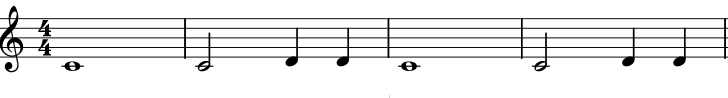
\includegraphics[scale=0.4]{thesis/obrazky-figures/copyvar.png}
    \caption{Variácia opakovaním.}
    \label{fig:copyvar}
    \end{figure}
    Aby sme mohli vytvoriť štvoricu taktov z obrázku \ref{fig:copyvar} musí derivácia vyzerať nasledovne: $$ (S) \Rightarrow_G (XX) $$ 
    $$\Rightarrow_G c1\_cXc1\_cX$$ 
    $$\Rightarrow_G c1\_cc1\_pXc1\_cc1\_pX$$ 
    $$\Rightarrow_G c1\_cc1\_pd1\_\check{s}Xc1\_cc1\_pd1\_\check{s}X$$ 
    $$\Rightarrow_G c1\_cc1\_pd1\_\check{s}d1\_\check{s}Xc1\_cc1\_pd1\_\check{s}d1\_\check{s}X$$
    $$\Rightarrow_G c1\_cc1\_pd1\_\check{s}d1\_\check{s}|c1\_cc1\_pd1\_\check{s}d1\_\check{s}|.$$
\end{example}

\begin{example}
Majme variáciu, ktorá zvýši tému o jeden tón.
\begin{figure}[H]
    \centering
    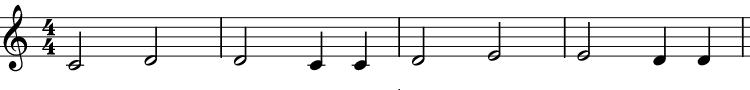
\includegraphics[scale=0.4]{thesis/obrazky-figures/sequp.png}
    \caption{Variácia zvýšením témy o jeden tón.}
    \label{fig:zvysenievar}
    \end{figure}
    Vytvorenie tejto variácie zo štvorice taktov \ref{fig:zvysenievar} je sprevádzané nasledujúcou deriváciou:
    $$ S \Rightarrow_G XX $$
    $$\Rightarrow_G  c1\_pXd1\_pX$$
    $$\Rightarrow_G  c1\_pd1\_pXd1\_pe1\_pX$$
    $$\Rightarrow_G  c1\_pd1\_pd1\_pXd1\_pe1\_pe1\_pX$$
    $$\Rightarrow_G  c1\_pd1\_pd1\_pd1\_\check{s}Xd1\_pe1\_pe1\_pd1\_\check{s}X$$
    $$\Rightarrow_G  c1\_pd1\_pd1\_pc1\_\check{s}c1\_\check{s}Xd1\_pe1\_pe1\_pd1\_\check{s}d1\_\check{s}X$$
    $$\Rightarrow_G  c1\_pd1\_pd1\_pc1\_\check{s}c1\_\check{s}|d1\_pe1\_pe1\_pd1\_\check{s}d1\_\check{s}|.$$
\end{example}

\begin{example}
Majme variáciu, ktorá zníži tému o jeden tón.
\begin{figure}[H]
    \centering
    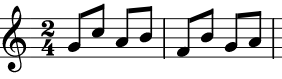
\includegraphics[scale=0.4]{thesis/obrazky-figures/seqdown.png}
    \caption{Variácia znížením témy o jeden tón.}
    \label{fig:znizenievar}
    \end{figure}
    Pre tvorbu variácie z obrázku \ref{fig:znizenievar} je zostavená derivácia:
    $$ S \Rightarrow_G XX $$
    $$\Rightarrow_G  g1\_oXf1\_oX$$
    $$\Rightarrow_G  g1\_oc2\_oXf1\_oh1\_oX$$
    $$\Rightarrow_G  g1\_oc2\_oa1\_oXf1\_oh1\_og1\_oX$$
    $$\Rightarrow_G  g1\_oc2\_oa1\_oh1\_oXf1\_oh1\_og1\_oa1\_oX$$
    $$\Rightarrow_G  g1\_oc2\_oa1\_oh1\_o|f1\_oh1\_og1\_oa1\_o|.$$
\end{example}

\begin{example}
Majme variáciu, ktorá predĺži tóny témy o polovicu.
\begin{figure}[H]
    \centering
    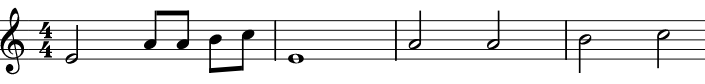
\includegraphics[scale=0.4]{thesis/obrazky-figures/augvar.png}
    \caption{Predĺženie dĺžky tónu o polovicu.}
    \label{fig:predlzenievar}
    \end{figure}
    Derivácia variácie z obrázku \ref{fig:predlzenievar} je nasledovná: 
    $$ S \Rightarrow_G XX $$
    $$\Rightarrow_G e1\_pXe1\_cX $$
    $$\Rightarrow_G e1\_pa1\_oXe1\_ca1\_\check{s}X $$
    $$\Rightarrow_G e1\_pa1\_oa1\_oXe1\_ca1\_\check{s}a1\_\check{s}X $$
    $$\Rightarrow_G e1\_pa1\_oa1\_oh1\_oXe1\_ca1\_\check{s}a1\_\check{s}h1\_\check{s}X $$
    $$\Rightarrow_G e1\_pa1\_oa1\_oh1\_oc2\_oXe1\_ca1\_\check{s}a1\_\check{s}h1\_\check{s}c2\_\check{s}X $$
    $$\Rightarrow_G e1\_pa1\_oa1\_oh1\_oc2\_o|e1\_ca1\_\check{s}a1\_\check{s}h1\_\check{s}c2\_\check{s}|.$$
\end{example}

\begin{example}
Majme variáciu, ktorá skráti dĺžku tónov témy.
\begin{figure}[H]
    \centering
    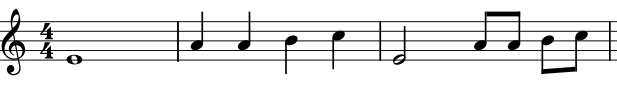
\includegraphics[scale=0.4]{thesis/obrazky-figures/dimivar.png}
    \caption{Skrátenie dĺžky tónu o polovicu.}
    \label{fig:skratenievar}
    \end{figure}
    Derivácia pre variáciu z obrázku \ref{fig:skratenievar} vyzerá nasledovne:
    $$ S \Rightarrow_G XX $$
    $$\Rightarrow_G e1\_cXe1\_pX $$
    $$\Rightarrow_G e1\_ca1\_\check{s}Xe1\_pa1\_oX $$
    $$\Rightarrow_G e1\_ca1\_\check{s}a1\_\check{s}Xe1\_pa1\_oa1\_oX $$
    $$\Rightarrow_G e1\_ca1\_\check{s}a1\_\check{s}h1\_\check{s}Xe1\_pa1\_oa1\_oh1\_oX $$
    $$\Rightarrow_G e1\_ca1\_\check{s}a1\_\check{s}h1\_\check{s}c2\_\check{s}Xe1\_pa1\_oa1\_oh1\_oc2\_oX $$
    $$\Rightarrow_G e1\_ca1\_\check{s}a1\_\check{s}h1\_\check{s}c2\_\check{s}|e1\_pa1\_oa1\_oh1\_oc2\_o|.$$
\end{example}

\begin{example}
Majme variáciu, ktorá vykoná transpozíciu témy.
\begin{figure}[H]
    \centering
    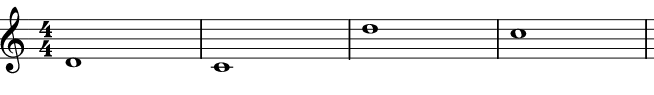
\includegraphics[scale=0.4]{thesis/obrazky-figures/transpos.png}
    \caption{Postupné zníženie témy o jeden tón.}
    \label{fig:transpovar}
    \end{figure}
    Derivácia pre transpozíciu z obrázku \ref{fig:transpovar} je nasledovná:
    $$ S \Rightarrow_G XX $$
    $$ \Rightarrow_G d1\_cXd2\_cX $$
    $$ \Rightarrow_G d1\_cc1\_cXd2\_cc2\_cX $$
    $$ \Rightarrow_G d1\_cc1\_c|d2\_cc2\_c| $$
\end{example}

\begin{example}
Majme variáciu, ktorá vykoná protipohyb témy.
\begin{figure}[H]
    \centering
    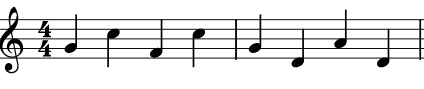
\includegraphics[scale=0.4]{thesis/obrazky-figures/contraryvar.png}
    \caption{Variácia protipohybom.}
    \label{fig:potrivar}
    \end{figure}
    Vzdialenosti pre variáciu protipohybom na obrázku sú $+3, -1, +3$. Vo výslednej variácií sú vzdialenosti oproti prvému tónu $-3, +1, -3$.
    $$ S \Rightarrow_G XX $$
    $$ \Rightarrow_G g1\_\check{s}Xg1\_\check{s}X $$
    $$ \Rightarrow_G g1\_\check{s}c2\_\check{s}Xg1\_\check{s}d1\_\check{s}X $$
    $$ \Rightarrow_G g1\_\check{s}c2\_\check{s}f1\_\check{s}Xg1\_\check{s}d1\_\check{s}a1\_\check{s}X $$
    $$ \Rightarrow_G g1\_\check{s}c2\_\check{s}f1\_\check{s}c2\_\check{s}Xg1\_\check{s}d1\_\check{s}a1\_\check{s}d1\_\check{s}X $$
    $$ \Rightarrow_G g1\_\check{s}c2\_\check{s}f1\_\check{s}c2\_\check{s}|g1\_\check{s}d1\_\check{s}a1\_\check{s}d1\_\check{s}| $$
\end{example}

\begin{example}
Majme variáciu, ktorá vykoná retrogradáciu témy.
\begin{figure}[H]
    \centering
    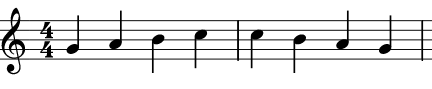
\includegraphics[scale=0.4]{thesis/obrazky-figures/retgradvar.png}
    \caption{Variácia retrogradáciou.}
    \label{fig:retrogradvar}
    \end{figure}
    Dvojica taktov na obrázku \ref{fig:retrogradvar} je vytvorená deriváciou:
    $$ S \Rightarrow_G R $$
    $$ \Rightarrow_G g1\_\check{s}Rg1\_\check{s} $$
    $$ \Rightarrow_G g1\_\check{s}a1\_\check{s}Ra1\_\check{s}g1\_\check{s}$$
    $$ \Rightarrow_G g1\_\check{s}a1\_\check{s}h1\_\check{s}Rh1\_\check{s}a1\_\check{s}g1\_\check{s}$$
    $$ \Rightarrow_G g1\_\check{s}a1\_\check{s}h1\_\check{s}c2\_\check{s}Rc2\_\check{s}h1\_\check{s}a1\_\check{s}g1\_\check{s}$$
    $$ \Rightarrow_G g1\_\check{s}a1\_\check{s}h1\_\check{s}c2\_\check{s}|c2\_\check{s}h1\_\check{s}a1\_\check{s}g1\_\check{s}$$
\end{example}

\section{Nelimitovaný hlboký zásobníkový automat}
Táto sekcia definuje nelimitovaný hlboký zásobníkový automat. Z jeho definície vychádzame pri návrhu tvorby algoritmu v nasledujúcej sekcii \ref{sec:alg}. Sekcia oboznamuje čitateľa s jeho využitím pri tvorbe variácií. Popisuje jeho novú verziu modelu, pomocou ktorého tvoríme variácie témy. Popisuje taktiež aj kľúčovú vlastnosť tohto automatu, ktorá je potrebná pre tvorbu variácií pomocou tohto automatu. Poznatky a definícia tohto automatu sú prevzaté z \cite{FITPUB10978}.

\subsection{Definícia}
\begin{definition}
Pod absolútne nelimitovaným zásobnikovým automatom rozumieme osmicu $M = (Q, \Sigma, \Gamma, \$, R, s, S, F)$, ktorá sa skladá z
\begin{itemize}\itemsep0.05em
\item konečnej množiny stavov $Q$,
\item vstupnej abecedy $\Sigma$,
\item zásobnikovej abecedy $\Gamma$,
\item množiny pravidiel $R$, ktoré sú konečnou reláciou $R \subseteq Q \times (\Gamma \setminus (\Sigma \cup \{\$\})) \times Q \times (\Gamma \setminus \{\$\})^* \times Q \times (\Gamma \setminus \{\$\})^*)\{\$\})$,
\item špecialneho symbolu $\$ \in \Gamma \setminus \Sigma$ pre spodok zásobnika,
\item počiatočného stavu $s \in Q$,
\item počiatočného zásobnikového symbolu $S \in \Gamma$,
\item množiny konečných stavov $F \subseteq Q.$
\end{itemize}
\end{definition}

Pravidlá nezapisujeme $(a, A, q, x) \in R$, ale ako $pA \rightarrow qx$. Majme reláciu ${}^a_p\vdash$ nad $Q \times \Sigma^* \times (\Gamma \setminus \{\$\})^*)\{\$\}$ takú, že $(p, aw, az) \, {}^a_p\vdash (p, w, z)$. Pre uvedené symboly platí $p \in Q, a \in \Sigma, w \in \Sigma^*$ a $z \in \Gamma^*$. Hovoríme potom o operácií zásobníka $pop$ pre $M$, ktorá odstráni $a \in \Sigma$ z $(p, aw, az)$ na $(p, w, z)$. Pod $(p, q, uAv) {}^a_\epsilon \vdash (p, q, uAv)[pA \rightarrow qx]$ rozumieme, že $M$ expanduje svoj zásobník s absolútne nelimitovanou expanziou z $(p, w, uAv)$ po $(q, w, uxv)$ na základe $pAv \rightarrow qx$.

Jazyk, ktorý $M$ prijíma pomocou prázdneho zásobníka, $L(M)_\epsilon$ je definovaný ako $$L(M)_\epsilon = \{w \in \Sigma^* \,| \, (s, w, S\$) {}^a\vdash^* (q, \epsilon, \$), kde \, q \in Q\}.$$. Tento spôsob využívame aj v tejto práci.

\subsection{Použitie a sila tvorby variácii}
Hlboký zásobníkový automat definovaný pozri \cite{FITPUB10498} je generalizáciou zásobníkového automatu \ref{def:zasaut}. Využitie hlbokého zásobníkového automatu spočíva v LL syntaktickej analýze. V nej môžeme vrchný symbol zásobníka buď expandovať alebo ho odstrániť. Vďaka hlbokému zásobníkovému automatu môžeme túto expanziu vykonávať vo vnútri tohto zásobníka. Týmto sme zvýšili akceptačnú silu zásoníkového automatu. Vďaka tejto vlastnosti môžeme LL prekladačmi spracovať kontextové jazyky. Samozrejme, že toto neplatí pre všetky kontextové jazyky, pretože hĺbka expanzie je limitovaná.

Aby mohol užívateľ tvoriť variácie z nami navrhnutej gramatiky \ref{mainalg}, budeme potrebovať hlboký zásobníkový automat. Dopredu však nepoznáme dĺžku reťazca, ktorý reprezentuje tému alebo celú skladbu. Aby sme mohli naďalej vytvárať variácie podľa našej gramatiky, budeme potrebovať nami definovaný absolútne nelimitovaný hlboký zásobníkový automat. Ten nás nelimituje v hĺbke expanzií, takže môžeme vytvárať variácie o ľubovoľnej dĺžke.

Expanzie absolútne nelimitovaného zásobníkového automatu sú prirodzenou generalizáciou n--limitovaného hlbokého zásobníku. Pomocou pravidiel, ktoré majú špecifikovaný najvrchnejší neterminál vieme expandovať nezávisle na jeho hĺbke. Toto nám umožňuje aplikovať krížové vlastností variácií a vytvárať ich tak. Sila tvorby týchto variácií, ktoré vytvárame pomocou absolútne nelimitovaných hlbokých expanzií je rovnaká lineárne ohraničenému automatu pre propagujúcu sa verziu. Taktiež má aj silu turingovho stroja pre mazacie verzie.

\subsection{Konštruovanie variácií}
Podobný princíp, ktorý je použitý pre prekladač sme prevzali z \cite{FITPUB10498}. Majme definovanú gramatiku pre tvorbu variácií \ref{mainalg}. Aby sme mohli tvoriť variácie na základe reťazca, ktorý zadal užívateľ, musíme zaviesť absolútne nelimitovaný hlboký zásobníkový automat $M$. Ten zavedieme tak, že pre každé pravidlo s rozptýleným kontextom $$(A_1, A_2, ..., A_n) \rightarrow (x_1, x_2, ..., x_n)$$ zavádzame pravidlá pre absolútne nelimitovaný zásobníkový automat $$sA_n \rightarrow s_{n-1}x_n,$$ $$s_{n-1}A_{n-1} \rightarrow s_{n-2}x_{n - 1},$$ $$\vdots$$ $$s_1A_1 \rightarrow sx_1.$$ M ma štartovný symbol $s$. Od $s_1$ po $s_{n - 1}$ máme nové unikátne stavy. M expanduje nevstupný symbol vo vnútri zásobníku, ktorým musí byť $A$. Expanzia $A$ na $x$ a presunutie sa do stavu q je podľa pravidla $pA \rightarrow qx$. Oproti hlbokému zásobníkovému automatu sme sa zbavili číslovania expanzií. Napriek tomu musíme dodržovať poradie expanzie, ktoré je uvedené vyššie. Ak by sme to nedodržali, tak by táto konštrukcia nefungovala správne.

\begin{table}[!ht]
\label{tabulLL}
\centering
\begin{tabular}{|l|l|l|}
\hline
  & c1\_c & | \\ \hline
S & 1     & 1 \\ \hline
X & 2/3   & 4\\ \hline
\end{tabular}
\caption{LL tabuľka}
\end{table}

Zostrojená tabuľka \ref{tabulLL} je ukážkou z gramatiky \ref{mainalg}. Očíslované pravidlá sú $$1: (S) \rightarrow (XX)$$$$2: (X,X) \rightarrow (c1\_cX, c1\_cX),3: (X,X) \rightarrow (c1\_cX, d1\_cX)$$$$4:(X,X) \rightarrow (|,|).$$ Vo výslednej tabuľke uvažujeme iba o netermináloch, ktoré sú na ľavej strane. Nerozhodnosť, ktorá nastala medzi pravidlami 2 a 3 je rozhodnutá užívateľom. Ak si užívateľ zvolil variáciu opakovaním, zvolí sa pravidlo 2 inak 3.

Tento spôsob tvorby variácií podľa užívateľa a dodržania poradia expanzie zásobníka nám zanecháva hotové variácie. Zamerajme sa na pravú stranu pravidla 3. Tá sa skladá z dvoch tónov c1\_c a d1\_c. Tón c1\_c reprezentuje tému a d1\_c je tónom variácie. Tento princíp je aplikovaný u všetkých pravidiel. Takýmto spôsobom nahrádzame tóny témy na vrchole zásobníka a nelimitovane expandujeme zásobník $M$ tónami variácie.

\section{Algoritmus}
\label{sec:alg}
Táto sekcia je venovaná návrhu algoritmu, vďaka ktorému budeme môcť pravidlami tvoriť výsledné variácie. Tento algoritmus je založený na poznatkoch z prác \cite{tablemusic, FITPUB10498}. Obe práce pracujú s iným spôsobom prekladania gramatík s rozptýleným kontextom. Ak hovoríme o využití oneskoreného vyhodnotenia, tak hovoríme o práci \cite{tablemusic}. Ďalším spôsobom je použitie dočasného poľa a hlbokého zásobníkového automatu. Výsledný algoritmus sa zabera práve týmto spôsobom.

Tento spôsob nám umožňuje expanziu nie len na vrchole zásobníka, ale i hlboko v jeho vnútri. V tomto prípade je potrebné, aby zásobník bol implementovaný pomocou obojstranne viazaného zoznamu.

Algoritmus, ktorý nám umožňuje tvoriť variácie je založený na preklade bezkontextových gramatik pozri \cite{FITPUB10524}. Počas tohto algoritmu pracujeme so zásobníkom ako obojstranne viazaným zoznamom. Každý symbol, ktorý vkladáme do zásobníka má tvar $ \langle Symbol \rangle $. Vstup pre tento algoritmus je zostrojená LL-tabuľka na základe gramatiky \ref{mainalg}. Ďalším vstupom je téma od užívateľa v podobe reťazca tokenov a požadované variácie.

Začiatok algoritmu (riadky 1--3) spočíva v inicializácií pomocných premenných. Jednou z nich je maximálny index poľa s variáciami, potom pozície pre pole variácií a vstupné tokeny. Poslednou pomocnou premennou je príznak pre expanziu vo vnútri zásobníka. Na riadku 4--5 máme inicializáciu samotného zásobníka a dočasného poľa.

Dočasné pole vieme limitovať dĺžkou 2. Je to vďaka tomu, že v jednom čase na základe našej gramatiky bude obsahovať maximálne odkazy na 2 neterminály. V poli každý element $i$ ukazuje na jeden neterminál vo vnútri zásobníku. Na začiatku algoritmu je pole inicializovane tak, aby ukazovalo na prvý neterminál S.

Ďalej sa program vo vnútri \texttt{while} slučky vetvy na tri časti. Prvá na riadkoch 8--17 zahrňuje situáciu, kedy sa na vrchole zásobníka objaví znak pre ukončenie témy. Tento stav naznačuje to, že sa buď blížime ku koncu tvorby variácií alebo prechádzame na tvorbu ďalšej variácie. Stav prechodu na ďalšiu variáciu detekujeme tým, že sme nevyčerpali všetky variácie podľa pomocnej premennej. Výslednu variáciu uložíme a pokračujeme v tvorbe ďalšej variácie. Ak ide o ukončenie celej tvorby posunieme pozíciu premennej, ktorá číta tokeny zo vstupného reťazca. Po tomto stave sa nachádza na vstupe koniec témy a na zásobníku koncový symbol. Nasleduje uloženie poslednej variácie a tak vyprázdnime zásobník.

Druhá časť 18--20 je o čosi jednoduchšia. Tu detekujeme na vrchole zásobníka terminál, ktorý nie je koncom témy. Tento terminál odstránime z vrcholu zásobníka pomocou jeho operácie \textit{pop}. Vrchol zásobníka sa nahradí ďalším symbolom.

Tretia časť 23--37 nastáva vtedy, keď sa na vrchole zásobníka nachádza neterminál. Prvým krokom je získanie aktuálnej variácie. Potom sa začne s hľadaním pravidla v LL--tabuľke. Hľadanie prebieha na základe neterminálu \textit{TOP\_P} na vrchole zásobníka a terminálu \textit{t}. Po získaní tohto pravidla je potrebné vybrať to, ktoré patrí k aktuálnej variácii. Ďalej mame podmienku, ktorá rozhoduje o expanzií zásobníka. Majme príznak pre expanziu zásobníka v hĺbke je nastavený na \textit{True}. Vyberieme z dočasného poľa pozíciu neterminálu z hĺbky zásobníka. Túto pozíciu odstránime z dočasného poľa. Neterminal na získanej pozícii nahradíme tónom variácie hlboko v zásobníku. Nastavíme príznak expanzie v hĺbke na \textit{False}. 

Ak je príznak nastavený na \textit{False}. Získame pozíciu z dočasného poľa, ktorou je neterminál na vrchole zásobníka. Odstránime adresu tohto neterminálu z dočasného poľa. Zmeníme tento neterminal na vrcholu zásobníka za pretočenú časť pravidla pre variáciu. V prípade, že aktuálna variácia je retrogradácia, potom neumožňujeme expanziu vo vnútri zásobníka.

V prípade variácie retrogradácia, je správanie sa tohto algoritmu podobné obyčajnému zásobníkovému automatu \ref{def:zasaut}. Je to vďaka tomu, že túto variáciu vieme popísať bezkontextovou gramatikou. Počas tejto variácie sa nevykonáva expanzia vo vnútri zásobníku (Alg. \ref{algoritmus1} Riad. 36-37).

Koniec algoritmu nastáva vtedy, keď sme došli na koniec pola zadaných variácií. Funkcia \textit{save\_variation} nam postupne uložila tóny požadovaných variácií. Vstupný reťazec je prijatý, inak nastáva chyba. Reťazec je prijatý ako prvá časť jazyka, pod druhými časťami tohto jazyka rozumieme nami vytvorené variácie.

\begin{algorithm}
\label{algoritmus1}
\SetNlSkip{-1em}
\caption{Tabuľkou riadené spracovanie gramatiky s rozptýleným kontextom}
\SetNlSty{}{}{:}
\KwIn{ LL tabuľka pre $G = (N, T, P, S);x \in T^*$; zvolené variácie }
\KwOut{ variácie pre $x$, kde $x \in L(G)\:a \:vari\acute{a}cie \in L(G)$, inak $chyba$}
\SetStartEndCondition{ }{}{}%
\SetKwProg{Fn}{def}{\string:}{}
\SetKwFunction{Range}{range}%%
\SetKw{KwTo}{in}\SetKwFor{For}{for}{\string:}{}%
\SetKwIF{If}{ElseIf}{Else}{if}{:}{elif}{else:}{}%
\SetKwFor{While}{while}{:}{fintq}%
\AlgoDontDisplayBlockMarkers\SetAlgoNoEnd\SetAlgoNoLine%
\Indp
\Indpp
\medskip
$var\_count := len(vari\acute{a}cie) - 1$\;
$var\_position,\, position := 0$\;
$deep\_push := False$\;
inicializácia zásobníka s $\langle \$ \rangle, \langle S \rangle$\;
inicializácia dočastného poľa s $pos\_S$\;
    \While{zasobník nie je prázdny} {
        nech $TOP\_P$ je vrchol zásobnika, t je momentálny token\;
        \uIf{$ TOP\_P = | $}{
            $var\_position += 1$\;
           \uIf{$ t = \$ $ a zároveň $var\_position > var\_count$}{
                $save\_variation()$\;
                $TOP\_P.pop()$
            }
            \uElseIf{$ t = | $ a zároveň $var\_position > var\_count$}{
                $position += 1$\;
            }
            \Else{
                $save\_variation()$\;
                $restart()$\;
            }
        }
        \uElseIf{$ TOP\_P \in T $}{
            \eIf{$ t = TOP\_P $}{
                $TOP\_P.pop()$\;
            }{
                $chyba$\;
            }
        }
        \uElseIf{$ TOP\_P \in N $}{
            $vari\acute{a}cia := get\_variation(var\_position)$\;
            $r := (X\_1, X\_2, \dots, X_n) \rightarrow (x_1, x_2, \dots. x_n) \in LL-tabu\check{l}ke[TOP\_P, t]$\;
            $pravidlo = r[vari\acute{a}cia]$\;
            \eIf{$deep\_push$}{
                $pos := do\check{c}as\_pole[0]$\;
                $do\check{c}as\_pole.remove(TOP\_P.pop())$\;
                vymeň v zasobniku pos za $preto\check{c}(pravidlo[2][1])$\;
                $deep\_push = False$\;
            }{
                $pos := do\check{c}as\_pole[0]$\;
                $do\check{c}as\_pole.remove(TOP\_P.pop())$\;
                vymeň TOP\_P za $preto\check{c}(pravidlo[2][0])$\;
                \If {$vari\acute{a}cia \neq retrograd\acute{a}cia$} {
                    $deep\_push = True$\;
                }
            }

        }
        \Else{
            $chyba$\;
        }
    }
\end{algorithm}

\chapter{Implementácia}
\label{chap:imp}
Kapitola implementácia sa zaoberá nami navrhnutým modelom pre tvorbu variácií. Implementácia tohto modelu vychádza z doteraz zozbieraných poznatkoch a vlastnostiach o bezkontextových, a kontextových gramatikách. Jadrom výslednej implementácie bude algoritmus \ref{algoritmus1}. Pravidla, ktoré budú aplikované vychádzajú z gramatiky \ref{mainalg}.

Najprv si rozoberieme technológie, ktoré sme si vybrali pre implementáciu. Zároveň uvedieme knižnicu, ktorá umožňuje prehrávanie výsledku. Potom zájdeme hlbšie, a to do štruktúry samotnej implementácie. Tá sa skladá z tried. Ďalej prezentujeme formát vstupu a výstupu, ktorý bol použitý pre reprezentáciu notového zápisu. Ako posledné si rozoberieme výsledky implementácie a jej porovnanie so zadanou témou.

\section{Použité technologie a knižnice}
\label{technologies}
Keďže predmetom tejto práce nie je kladený dôraz na rýchlosť prekladu, tak bol k implementácií použitý jazyk Python. Python je interpretovaný, objektovo orientovaný, dynamický typovaný a vysoko úrovňový programovací jazyk. Oproti jazykom akým je jazyk C alebo C++ postráda rýchlosť prekladu. Tá je kľúčová k implementácií prekladačov nových programovacích jazykov. Programovací jazyk python na oplátku ponúka jednoduchý syntax, obrovský výber a jednoduchú manipuláciu s balíkmi. Viac o tomto jazyku v \cite{python:site}.

Mimo štandardných balíčkov, implementovaný program používa jeden balíček, ktorý je pod všeobecnou verejnou licenciou. Ide o syntezátor, ktorého použitie si môže zvoliť užívateľ na prehrávanie výsledku tvorby variácií. Vďaka nemu si môže človek neznalý notového zápisu prehrať výsledne variácie. Ide o virtuálny analógový syntezátor. Návod na jeho manipuláciu a ukážky použitia môžeme nájsť v \cite{synt:site}.

\section{Vstup a výstup}
\label{inputoutput}
Vstup aj výstup programu je vo formáte XML. Tento princíp je prevzatý z \cite{afrpub}. Tento formát nám umožňuje reprezentovať určitým spôsobom notový zápis. Tento formát sa skladá z elementov, ktorým vieme pripísať rôzne atribúty. To sa nám hodí pri popise notového zápisu, keďže jednotlivé tóny majú svoje atribúty. Notový zápis sa skladá taktiež z rôznych elementov (tónov) a atribútov (dĺžka). Príklad vstupného súboru je nasledujúci.
\newpage
\lstset{language=XML}
\begin{lstlisting}
<theme time_signature="3/4">
    <measure>
        <tone note="half">c1</tone>
        <tone note="eight">d1</tone>
        <tone note="eight">e1</tone>
    </measure>
</theme>
\end{lstlisting}

Vstupný súbor obsahuje koreňový element \textit{theme}. Tento element musí obsahovať atribút s predpisom dĺžky taktu \textit{time\_signature}. Aby sme predišli nezmyselným konštrukciám, tak sme tento atribút obmedzili na hodnoty 2/4, 3/4 a 4/4. Tieto predpisy taktov sú v hudbe najrozšírenejšie.

Vo vnútri koreňového elementu sú elementy \textit{measure}. Ide o element pre takt. Ten obsahuje elementy pre jednotlivé tóny nazývane \textit{tone}.

V notovom zápise je počet elementov \textit{tone} závislí od taktového predpisu, ktorý je v tomto súbore 3/4. Tento element má atribút \textit{note}, ktorý popisuje dĺžku tónu. Aby sme si overili dĺžku uvedeného elementu \textit{measure}, potrebujeme spočítať dĺžky tónov v atribúte \textit{note}. Maximálny počet dôb v takte je podľa \textit{time\_signature} 3. Zo štvorky vyčítame trvanie štvrťovej noty, ktoré je jednu dobu. Potom výpočet je nasledovný $2 + 1/2 + 1/2 = 3.$ Polovicu doby trvá osminová nota, pretože štvrťová nota trvá jednu dobu. Textom elementov \textit{tone} je názov tónu.

Na podobnom princípe je založený aj formát výstupu. Ten sa skladá z koreňového elementu \textit{variations}. Vo vnútri tohto koreňového elementu sú zahrnuté všetky výsledné variácie. Tie sú zoradené podľa zoznamu argumentov uvedenom v podsekcii \ref{args}.

\lstset{language=XML}
\begin{lstlisting}
<?xml version="1.0" ?>
<variations>
	<variation>
		<measure>
			<tone note="half">c1</tone>
			<tone note="eighth">d1</tone>
			<tone note="eighth">e1</tone>
		</measure>
	</variation>
</variations>
\end{lstlisting}

\section{Prehľad tried}
Výsledná implementácia využíva objektovo orientované programovanie. Štruktúra programu je rozdelená do tried. Tieto triedy vykonávajú rôzne činnosti, ako sú spracovanie argumentov, extrahovanie vstupu, tvorby variácií, prehrávanie variácií a vytvorenie výstupu.

\subsection{Argumenty}
\label{args}
Pomocou argumentov si užívateľ môže zvoliť variácie, ktoré sa budú vytvárať. Spracovanie argumentov zabezpečuje trieda \textit{ArgParser}. Hlavnou metódou tejto triedy je \textit{parse}. Cieľom tejto metódy je overiť správnosť argumentov a uložiť zadané argumenty pre ďalšie spracovanie. Jednotlivé variácie majú pridelené nasledujúce argumenty:

\begin{itemize}\itemsep0.05em
    \item -r, -{}-repetition pre variáciu opakovanim
    \item -t, -{}-transposition pre variáciu transpozíciou
    \item -S, -{}-sequence-up pre postupne zvyšovanie o jeden tón
    \item -s, -{}-sequence-down pre postupne zníženie o jeden tón
    \item -c, -{}-contrary\_motion pre variáciu proti pohybom
    \item -R, -{}-retro\_gradation pre variáciu retrogradáciou
    \item -a, -{}-augmentation pre variáciu zdvojnásobenia dĺžky tónov
    \item -d, -{}-diminution pre variáciu skrátenia dĺžky tónov o polovicu
\end{itemize}

Tieto argumenty patria všetkým variáciám, ktoré sme si navrhli a podarilo sa ich implementovať. Keďže sa pohybujeme na jednočiarkovanej a dvojčiarkovanej oktáve, nie všetky variácie sa môžu vykonávať viackrát pre jednu tému. Tie, ktoré vieme vykonať viackrát sú zvýšenie a zníženie témy o jeden tón. Patria pre ne obmedzenia, že sa môžu vykonať iba pre jednu oktávu. Takže pre tieto argumenty vieme zadať počet vykonaní od 1 po 7 vrátane. Ostatné argumenty iba povolia vykonanie príslušnej variácie. Argumenty

\begin{itemize}\itemsep0.05em
    \item -p, -{}-play 
    \item -{}-save
    \item -v, -{}-volume
\end{itemize}

súvisia s použitou knižnicou syntetizátora. Argument \textit{-p} prehrá výsledné variácie, \textit{save} uloží výsledok variácií do súboru pre prehratie a \textit{v} nastaví hlasitosť výstupu. Argument -i a -{}-input umožňuje zadať vstupný súbor vo formáte xml.

\subsection{Spracovanie vstupu}
Spracovanie vstupu zabezpečuje trieda \textit{InputExtractor}. Jej úlohou je spracovať vstup zadaný užívateľom. Formát tohto vstupu je rozoberaný v \ref{inputoutput}. 

Hlavnou metódou tejto triedy je \textit{read\_input}. Pomocou nej čítame vstup, z ktorého potrebujeme predpis taktov. Ten je potrebný pre formatovanie výstupu. Ďalej z elementov vo vstupnom súbore vyberie dĺžky tónov a ich názvy. Toto uskutočňuje pomocou metódy \textit{fill\_list}. Dvojice tón a dĺžka sú uložené do slovníka pre tvorbu variácií.

\subsection{Zásobník}
Aby sme mohli zásobník expandovať v nejakej hĺbke, potrebujeme ho implementovať pomocou obojstranne viazaného zoznamu. Informácie a časť metód pre obojstranne viazaný zoznam boli prevzaté z \cite{dll:site}.

Implementácia zásobníka sa nachádza v súbore \textit{DLL.py}. Súbor sa skladá z dvoch tried \textit{Node} a \textit{DLL}.

Trieda \textit{Node} znázorňuje symbol v zásobníku. Tým môže byť hociktorý zo zásobníkovej abecedy. Súčasťou tohto symbolu sú odkazy na nasledujúci symbol a predchádzajúci symbol. Dôležitými operáciami tohto zásobníka sú:

\subsubsection*{def push(data)}
Pomocou tejto operácie vkladáme prvé častí z pravých strán pravidiel LL gramatiky s rozptýleným kontextom. Tie sú vkladané na vrch zásobníka. Pod nimi rozumieme tóny hlavnej témy alebo skladby, ktorú chce užívateľ variovať.

\subsubsection*{def pop()}
Vložené tóny na vrchu zásobníka sú rovnaké ako tie, ktoré si zadal užívateľ. Tie sú postupne z vrchu zásobníka odstraňované. Týmto spôsobom sa vyhneme tomu, že by výsledné variácie obsahovali tóny témy. Metóda nahradí na vrchu zásobníka nasledujúci symbol. Odkaz odstráneného symbolu je vráteny touto metódou.

\subsubsection*{def insert(prev\_node, data)}
Pomocou operácie \textit{insert} máme možnosť expandovať zásobník i v jeho hĺbke. To nám umožňuje vložiť tóny variácie do vnútra zásobníka. Vkladané sú pravidlá variácie, ktoré sú súčasťou druhej časti pravej strany pravidiel LL gramatiky s rozptýleným kontextom. Tie sú ukladané za neterminál, ktorý je hĺbke zásobníka. Odkaz za tento neterminal je v parametri tejto metódy \textit{prev\_node}. Pomocou parametru \textit{data} predáme symbol na vloženie.

\subsubsection*{def remove(node)}
Aby sme mohli odstrániť neterminály v hĺbke zásobníka používame operáciu \textit{remove}. Pre nahradenie neterminálu v hĺbke zásobníka musíme odstrániť po operácií \textit{insert} neaktuálny neterminal. Adresa starého neterminálu je predaná parametrom \textit{node} z dočasného poľa.

\subsubsection*{def printList(), def dll\_len()}
Trieda \textit{DLL} obsahuje ďalšie pomocné metódy, ako sú \textit{not\_empty} pre zistenie či zásobník nie je prázdny. Obsahuje vypísanie obsahu \textit{printList} a \textit{dll\_len} na získanie počtu symbolov v zásobníku.

\subsection{Tvorba variácií}
Tvorba variácií je sústredená do triedy \textit{CSGparser}. Atribútmi tejto triedy sú tokeny podľa tabuľky \ref{tab:tone}. Ďalej kompletná LL tabuľka na základe gramatiky \ref{mainalg} a kompletný zoznam pravidiel. Tento kompletný zoznam pravidiel je uložený v poli \textit{rules}.

\subsubsection*{def tokenizer()}
Úlohou tejto metódy je tvoriť tokeny, ktoré sa skladajú z názvu tónu a jeho dĺžky. Ukladajú sa postupne do poľa \textit{tokens}. Ich tvar je definovaný atribútmi triedy. Tieto tokeny sa tvoria zo slovníka, ktorý je vytvorený triedou \textit{InputExtractor}. Na konci tohto procesu sa priložia tokeny pre taktovú čiaru a symbol, ktorý značí koniec tohto reťazca tokenov. Návratová hodnota je výsledný reťazec tokenov.

\subsubsection*{Metody pre prácu s pravidlami a tabuľkou}
Aby sme mohli aplikovať pravidla podla algoritmu \ref{algoritmus1}, museli sme zaviesť rôzne operácie nad LL tabuľkou.

Jednou z nich je \textit{get\_rule}. Táto metóda vyberie bunku z tabuľky na základe vstupného tokenu, ktorý zadal užívateľ a vrchného symbolu na zábobníku. Vo vnútri tejto bunky sú priradené pravidlá podľa variácie. Aby sme mohli vybrať správne pravidlo pre požadovanú variáciu máme metódy \textit{get\_key} a \textit{get\_rule\_number}. Tieto metódy zvolia presné pravidlo pre variáciu z bunky tabuľky.

Pracujeme s obmedzenou množinou tónov, preto nemôžeme využiť plný potenciál pravidiel variácií. Ak nejaké pravidlo variácie presahuje túto množinu, tak sa zvoli pravidlo pre opakovanie tónu. Tieto vzťahy sú dopredu zavedené v LL tabuľke.

\subsubsection*{def reverse\_push(items, deep, nonterminal)}
Pomocou tejto metódy vieme pretočiť obsah pravej strany pravidiel LL gramatiky s rozptýleným kontextom. Tento otočený obsah pravidiel vkladáme do zásobníka. Vkladanie prebieha buď do hĺbky alebo na vrch zásobníka. Keďže pravidlá sa skladajú z n-tíc, ktoré sa nedajú metódami otočiť, tak sme použili radu z \cite{stack:site}. Pod parametrom \textit{items} rozumieme obsah, ktorý sa vkladá do zásobníka. Odkaz na neterminál v zásobníku z dočasného poľa je \textit{nonterminal} a \textit{deep} rozhoduje o vkladaní do hĺbky.

\subsubsection*{def save\_result(), def restart()}
Obe metódy spolu úzko súvisia. Aby sme mohli uložiť jednotlivé úseky variácií, tak používame metódu \textit{save\_result}. Tá na konci zozbiera tóny vytvorenej variácie zo zásobníka a uloží ich. Aby sme mohli tvoriť ďalšie variácie, tak potrebujeme vynulovať pozície čítania vstupu od užívateľa. To robíme pomocou metódy \textit{restart}. V prípade, že bol zadaný väčší počet variácií zvyšovania a znižovania tónov témy, potom sa variácie netvoria z témy. Tieto nasledujúce variácie sa tvoria z poslednej variácie zvyšovania a znižovania tónu.

\subsubsection*{def get\_distances(tokens)}
Aby sme mohli tvoriť variácie protipohybom, je potrebné získať vzdialenosti tónov zo vstupu. Tieto vzdialenosti sa počítajú na základe prvého tónu pre celú variáciu. Vzdialenosti sa vypočítajú vzorcom: $$vzdialenos\check{t} = (prv\acute{y}\_t\acute{o}n\_poz - t\acute{o}n\_poz) * 2.$$ Kde $prv\acute{y}\_t\acute{o}n\_poz$ je pozícia prvého tónu témy v poli $tuple\_list$ a $t\acute{o}n\_poz$ je pozícia každého ďalšieho tónu témy.

\begin{example}
Majme tému z tónov f a e. Pozícia tónu f je 3 a pozícia tónu e je 2. Potom $$(3 - 2) * 2 = 2.$$ Výsledna variácia bude musieť posunúť tón e o 2 pozície hore. Preto výsledna variácia sa skladá z tónov f a g.
\end{example}

Návratová hodnota je zoznam týchto vzdialenosti. Tie sa použijú pri zadanej variácií protipohyb. Variácia protipohybom je tá, ktorá obsahuje najviac pravidiel gramatiky. Je to preto, že tu sa krížiace sa závislosti riadia vzdialenosťami tónov. Tie posúvajú tón hore o rovnakú dĺžku, ako ho posúvajú dole.

\subsubsection*{def variator()}
Táto metóda je implementáciou algoritmu \ref{algoritmus1}. Tvorí výsledné variácie, ktoré sa ukladajú do atribútu triedy \textit{CSGparser}. Implementácia algoritmu je rozšírená o list vzdialenosti tónov pre variáciu protipohybom. 

\subsection{Prehranie výstupu a jeho výpis}
Aby si užívateľ mohol prehrať vytvorené variácie, tak sme vytvorili triedu \textit{TonesPlayer}. Cieľom tejto triedy je vytvoriť sínusové vlny podľa frekvencií, ktoré sme prevzali z \cite{strankaFrekvencii}. Trvanie týchto vĺn je určené podľa dĺžky nôt, ktoré sú vo variácií. Aby sme mohli toto všetko prehrať a vytvoriť, použili sme knižnicu, ktorú sme rozoberali v sekcii \ref{technologies}. Tieto výsledky je možné prehrať, ale i uložiť do súboru s príponou \textit{.wav}. Tento súbor sa uloží do rovnakého priečinku ako vstupný súbor.

O vypísanie výsledných variácii sa stará trieda \textit{Generator}. Formát tohto výstupu sme rozoberali v sekcii \ref{inputoutput}. Výstupný xml formát je ešte formatovaný tak, aby nebol vypísaný na jednom riadku. O to sa stará knižnica \textit{mini.dom}.

\section{Výsledky a porovnanie}
V tejto sekcií si predvedieme výsledky našej implementácie. Ukážeme si tému (vstup) a pre ňu vytvorené variácie (výstupy). Naša téma je jednoduchá a skladá sa z troch taktov. Zápis témy v notovom zápise s jej ekvivalentným zápisom v xml je nasledovný.

\begin{minipage}{0.45\textwidth}
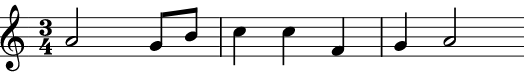
\includegraphics[width=\textwidth]{thesis/obrazky-figures/theme.png}
\end{minipage}%
\begin{minipage}{0.5\textwidth}
\centering
\lstset{language=XML}
\begin{lstlisting}[basicstyle=\tiny]
<theme time_signature="3/4">
    <measure>
        <tone note="half">a1</tone>
        <tone note="eight">g1</tone>
        <tone note="eight">h1</tone>
    </measure>
    <measure>
        <tone note="quarter">c2</tone>
        <tone note="quarter">c2</tone>
        <tone note="quarter">f1</tone>
    </measure>
    <measure>
        <tone note="quarter">g1</tone>
        <tone note="half">a1</tone>
    </measure>
</theme>
\end{lstlisting}
\end{minipage}

Ako prvú variáciu vytvoríme opakovanie témy. Táto variácia vznikla prekopírovaním tónov témy. Keď ju porovnáme s našou témou môžeme vidieť, že variácia sa vytvorila správne. Tóny variácie sú rovnaké ako tóny témy. Súčasťou tejto variácie sú krížiace sa závislosti so zadanou témou. Tie sme si znázornili na pravej strane obrázku \ref{fig:dependencies}. Spozorovať ich môžeme aj u ostatných variáciách až na retrogradáciu. Výsledok programu vo formáte xml a v notovom zápise je:

\begin{minipage}{.45\textwidth}
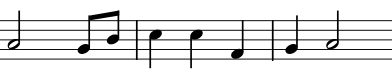
\includegraphics[width=\textwidth]{thesis/obrazky-figures/var1.png}
\end{minipage}%
\begin{minipage}{.5\textwidth}
\centering
\lstset{language=XML}
\begin{lstlisting}[basicstyle=\tiny]
<variation>
    <measure>
        <tone note="half">a1</tone>
        <tone note="eighth">g1</tone>
        <tone note="eighth">h1</tone>
    </measure>
    <measure>
        <tone note="quarter">c2</tone>
        <tone note="quarter">c2</tone>
        <tone note="quarter">f1</tone>
    </measure>
    <measure>
        <tone note="quarter">g1</tone>
        <tone note="half">a1</tone>
    </measure>
</variation>.
\end{lstlisting}
\end{minipage}

Druhá variácia, ktorá bola vytvorená je transpozícia. Pomocou tejto variácie sme preniesli našu tému o oktávu vyššie. Ak porovnáme výsledok tejto variácie s témou, tak môžeme vidieť tóny z témy. Rozdiel je ten, že sú v dvojčarikovanej oktáve. Naša téma sa nachádza v jednočiarkovanej oktáve. Odčítať tento výsledok z notového zápisu môžeme z obrázku \ref{fig:tonfrek}.

\begin{minipage}{.45\textwidth}
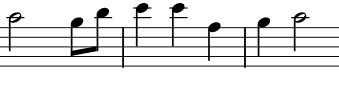
\includegraphics[width=\textwidth]{thesis/obrazky-figures/var22.png}
\end{minipage}%
\begin{minipage}{.5\textwidth}
\centering
\lstset{language=XML}
\begin{lstlisting}[basicstyle=\tiny]
<variation>
    <measure>
        <tone note="half">a2</tone>
        <tone note="eighth">g2</tone>
        <tone note="eighth">h2</tone>
    </measure>
    <measure>
        <tone note="quarter">c3</tone>
        <tone note="quarter">c3</tone>
        <tone note="quarter">f2</tone>
    <measure>
        <tone note="quarter">g2</tone>
        <tone note="half">a2</tone>
    </measure>
</variation>
\end{lstlisting}
\end{minipage}

Nasledujúci výsledok je variácia postupným zvýšením tónu. Výsledné zvýšenie témy je o jeden tón. Túto variáciu sme vykonali jeden krát. Zoberme si tóny variácie a témy. Z \ref{fig:tonfrek} vieme vyčítať, že variácia prebehla úspešne. Overiť môžme výsledok aj sluchom. Vypočuť si tak môžeme stúpavú melódiu našej témy.

\begin{minipage}{.45\textwidth}
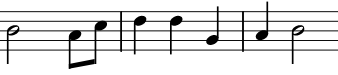
\includegraphics[width=\textwidth]{thesis/obrazky-figures/var3.png}
\end{minipage}%
\begin{minipage}{.5\textwidth}

\lstset{language=XML}
\begin{lstlisting}[basicstyle=\tiny]
<variation>
    <measure>
        <tone note="half">h1</tone>
        <tone note="eighth">a1</tone>
        <tone note="eighth">c2</tone>
    </measure>
    <measure>
        <tone note="quarter">d2</tone>
        <tone note="quarter">d2</tone>
        <tone note="quarter">g1</tone>
    </measure>
    <measure>
        <tone note="quarter">a1</tone>
        <tone note="half">h1</tone>
    </measure>
</variation>
\end{lstlisting}
\end{minipage}

Ďalšia variácia je zníženie témy o jeden tón. Na základe porovnania témy a výsledku vieme z taktového zápisu, že sme znížili tému o jeden tón. Tento výsledok vieme overiť aj sluchovo. Tak zistíme, že naša téma postupne klesá. Ak by sme nepracovali ohraničené na jednočiarkovanej a dvojčiarkovanej oktáve, tak by táto variácia pre nejaké n mohla klesať ešte nižšie. To by platilo pre frekvencie, ktoré vieme zachytiť sluchom.

\begin{minipage}{.45\textwidth}
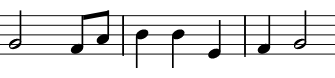
\includegraphics[width=\textwidth]{thesis/obrazky-figures/var4.png}
\end{minipage}%
\begin{minipage}{.5\textwidth}
\centering
\lstset{language=XML}
\begin{lstlisting}[basicstyle=\tiny]
<variation>
    <measure>
        <tone note="half">g1</tone>
        <tone note="eighth">f1</tone>
        <tone note="eighth">a1</tone>
    </measure>
    <measure>
        <tone note="quarter">h1</tone>
        <tone note="quarter">h1</tone>
        <tone note="quarter">e1</tone>
    </measure>
    <measure>
        <tone note="quarter">f1</tone>
        <tone note="half">g1</tone>
    </measure>
</variation>
\end{lstlisting}
\end{minipage}

Nasleduje výsledok pre variáciu protipohybom. Aby sme ju mohli vytvoriť, uvažovali sme vzdialenosti tónov z témy -1, +1, +2, +2, -2, -1 a 0. Výsledné vzdialenosti sú +1, -1, -2, -2, -2, +1 a 0. Môžeme si všimnúť piatu pozíciu, ktorá sa nezmenila. Je to tak, pretože náš systém posúva tóny dole o hodnotu, ktorú môže posunúť tóny aj hore. Keďže toto nemôžeme vykonať, tak tento tón nemeníme. Uplatnilo sa tak pravidlo opakovania.

\begin{minipage}{.45\textwidth}
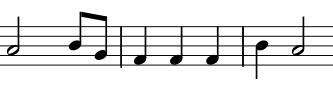
\includegraphics[width=\textwidth]{thesis/obrazky-figures/var5.png}
\end{minipage}%
\begin{minipage}{.5\textwidth}
\centering
\lstset{language=XML}
\begin{lstlisting}[basicstyle=\tiny]
<variation>
    <measure>
        <tone note="half">a1</tone>
        <tone note="eighth">h1</tone>
        <tone note="eighth">g1</tone>
    </measure>
    <measure>
        <tone note="quarter">f1</tone>
        <tone note="quarter">f1</tone>
        <tone note="quarter">f1</tone>
    </measure>
    <measure>
        <tone note="quarter">h1</tone>
        <tone note="half">a1</tone>
    </measure>
</variation>
\end{lstlisting}
\end{minipage}

Preklopenie témy, ktoré sme vytvorili variáciou témy je ďalším výsledkom. Ak ju porovnáme s témou vidíme, že sa začína od jej konca. Takto sme vytvorili vnorené závislosti, ktoré sú typické pre bezkontextové jazyky. Ich znázornenie môžeme nájsť na ľavej strane obrázku \ref{fig:dependencies}. Výsledok je na nasledujúcom obrázku.

\begin{minipage}{.45\textwidth}
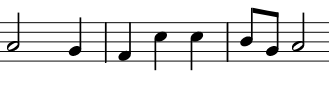
\includegraphics[width=\textwidth]{thesis/obrazky-figures/var7.png}
\end{minipage}%
\begin{minipage}{.5\textwidth}
\centering
\lstset{language=XML}
\begin{lstlisting}[basicstyle=\tiny]
<variation>
    <measure>
        <tone note="half">a1</tone>
        <tone note="quarter">g1</tone>
    </measure>
    <measure>
        <tone note="quarter">f1</tone>
        <tone note="quarter">c2</tone>
        <tone note="quarter">c2</tone>
    </measure>
    <measure>
        <tone note="eighth">h1</tone>
        <tone note="eighth">g1</tone>
        <tone note="half">a1</tone>
    </measure>
</variation>
\end{lstlisting}
\end{minipage}

Posledne dve variácie, ktoré vieme vytvoriť manipulujú s dĺžkami nôt našej témy. Nasledujúca variácia úspešne predĺžila dĺžky nôt témy. Samotné tóny témy sa zachovali. Počet taktov sa rozšíril, keďže dĺžky tónov by sme do pôvodného počtu taktov nezmestili.

\begin{minipage}{.46\textwidth}
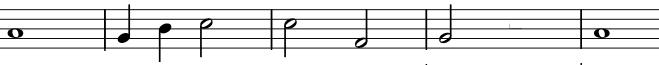
\includegraphics[width=\textwidth]{thesis/obrazky-figures/var8.png}
\end{minipage}%
\begin{minipage}{.5\textwidth}
\centering
\lstset{language=XML}
\begin{lstlisting}[basicstyle=\tiny]
<variation>
    <measure>
        <tone note="full">a1</tone>
    </measure>
    <measure>
        <tone note="quarter">g1</tone>
        <tone note="quarter">h1</tone>
        <tone note="half">c2</tone>
    </measure>
    <measure>
        <tone note="half">c2</tone>
        <tone note="half">f1</tone>
    </measure>
    <measure>
        <tone note="half">g1</tone>
        <tone note="full">a1</tone>
    </measure>
</variation>
\end{lstlisting}
\end{minipage}

Opakom predchádzajúcej variácie je skrátenie dĺžky tónov témy. U tejto variácie sa dĺžka nôt skrátila natoľko, že sme ich mohli vložiť iba do dvoch taktov. V porovnaní s témou sme tóny zachovali, zmenili sme však dĺžky nôt. Dĺžku nôt témy sme skrátili na polovicu.

\begin{minipage}{.45\textwidth}
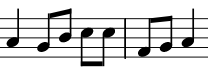
\includegraphics[width=\textwidth]{thesis/obrazky-figures/var9.png}
\end{minipage}%
\begin{minipage}{.5\textwidth}
\centering
\lstset{language=XML}
\begin{lstlisting}[basicstyle=\tiny]
<variation>
    <measure>
        <tone note="quarter">a1</tone>
        <tone note="eighth">g1</tone>
        <tone note="eighth">h1</tone>
        <tone note="eighth">c2</tone>
        <tone note="eighth">c2</tone>
    </measure>
    <measure>
        <tone note="eighth">f1</tone>
        <tone note="eighth">g1</tone>
        <tone note="quarter">a1</tone>
    </measure>
</variation>
\end{lstlisting}
\end{minipage}

\chapter{Záver}
\label{chap:end}
\section{Dosiahnuté výsledky}
Predmetom práce bolo zoznámiť sa s rôznymi formálnymi modelmi. Jedným z nich, ktoré našli uplatnenie v hudbe sú Markovovské procesy. Uplatnenie týchto modelov môžeme nájsť v práci \cite{afrpub}. Taktiež by sme vedeli nájsť rôzne uplatnenia pre automaty a gramatiky, ktoré sú rozoberané v tejto práci. Z pozorovania vyplynulo, že rôzne vlastností gramatík a automatov umožňujú popísať, a postupne pravidlami tvoriť rôzne druhy hudobných konštrukcií.

Štúdiom hudobných konštrukcii a úsekov sme zistili, že tie, ktoré by sme vedeli popísať formálnymi modelmi sú téma a jej variácie. Variácie, ktoré boli použité pre výsledné modely pochádzajú z sématického rozpoznávania hudobných objektov. Tieto variácie sú opakovanie, transpozícia, postupnosť, protipohyb, retrogradácia, predĺženie a skrátenie dĺžky tónu. Študovali sme tieto variácie. Hľadaním spôsobu, ako popísať tieto konštrukcie formálnymi modelmi sme zistili, že vhodný formálny model sú gramatiky. Rôzne variácie, ktoré sú zapísané v notovom zápise sa ukázali ako reťazce. Tieto reťazce vykazujú vlastnosti, ktoré vieme popísať bezkontextovými a kontextovými jazykmi. Hovoríme o vnorených závislostiach pre bezkontextové jazyky a krížiace sa závislosti pre kontextové jazyky. Variácia retrogradácia ukázala tvorbu hudobných reťazcov vnorenými závislosťami medzi tónmi. Výsledkom tohto pozorovania je bezkontextová gramatika, ktorá pravidlami popisuje túto konštrukciu. Vďaka tejto gramatike sme pravidlami vytvorili variáciu retrogradácia. Ostatné variácie sa ukázali ako nepopísateľné bezkotextovými gramatikami. Aby sme mohli ostatné variácie tvoriť museli sme zájsť do kontextových gramatik.

Kontextové gramatiky sú silnejší formalizmus akým sú bezkontextové gramatiky. Vďaka tomu sme mohli do nej zahrnúť aj tvorbu retrogradácie, ktorá je bezkotextova. Štúdium rôznych kontextových gramatík, ktoré by mohli byť vhodné pre tvorbu hudobnej štruktúry ukázalo, že vhodnou gramatikou bude gramatika s rozptýleným kontextom. Existujúce aplikácie gramatiky s rozptýleným kontextom v lingvistike ukázali možnosť generovania gramatických viet. Tento princíp sme uplatnili v hudbe. Preskočenie kontextu v hudbe nám umožnilo generovať rôzne reťazce. Pod týmito reťazcami chápeme variácie témy. Tieto variácie vytvárame programovo vstupom užívateľa. Zostavili sme teda prekladač na základe LL gramatiky s rozptýleným kontextom a absolútne nelimitovaným hlbokým zásobníkovým automatom. Ten nám umožní spracovať vstupný reťazec, ktorý je téma. Počas tohto procesu vytvorí variáciu k tejto téme. Tento proces je potrebný, pretože spolu tvoria jednu štruktúru. Výsledná LL tabuľka sa skladá z pravidiel, ktoré znázorňujú tvorbu jednotlivých križiacich sa závislosti vo variáciách. Výsledná tabuľka by bola nerozhodnuteľná, ale vďaka tomu, že rozlišujeme pravidlá pre jednotlivé variácie, tak vieme zvoliť výsledné pravidlo pre konkrétnu variáciu.

Na základe týchto výsledkov sme si mohli zaviesť novú verziu modelu, ktorý je založený na LL gramatike s rozptýleným kontextom. Výsledkom tohto modelu je tvorba zvolenej variácie na základe vstupnej témy od užívateľa. Tento model sme implementovali v jazyku python. Pre správny chod tejto aplikácie je potrebný vstupný súbor vo formáte xml. Xml formát je použitý na reprezentáciu nôt pomocou elementov, a ich atribútov. Tento formát je vhodný aj pre výstup, ktorým sú pravidlami vyprodukované variácie. Jadro výslednej implementácie sa skladá z LL tabuľky, ktorá obsahuje pravidlá LL gramatiky s rozptýleným kontextom. Skladanie variácie je riadené nekonečným hlbokým zásobníkom, vďaka ktorému môžeme neustále rozširovať zásobník v hĺbke. Výsledné použitie tohto zásobníku leží v tom, že aplikuje prvú časť pravej strany pravidla ako pravidlo témy, a hlboko do zásobníka pravidlo variácie tónu z témy.

Dosiahnutý výsledok tejto práce spočíva vo variovaní rôznych tém, ktoré zadá užívateľ. Na základe vytvorených výstupov si vie pozrieť zápis, ale aj vypočuť výsledné variácie. To mu zjednoduší rozhodovanie o tom, ktorú variáciu použije a či ju použije vo výslednej skladbe. Zjednodušenie je aj v tom, že užívateľ nemusí odchádzať od počítača k overeniu si svojej predstavy na hudobnom nástroji. Nemusí si taktiež ani zapisovať variáciu aby si ju následne overil. Výsledok je zapísaný vo formáte xml. Ten sa jednoducho spracováva rôznymi knižnicami. Výsledok sa dá použiť k obmieňaniu hudby v počítačových hrách. Hudba v týchto hrách sa skladá z rôznych melódií. Táto práca ich vie variovať a priniesť tak rozmanitejší zážitok z hudby v hrách.

\section{Ďalší vývoj}
Ďalší vývoj tohto projektu sa môže uberať viacerými smermi. Jedným z nich môže byť zbieraním podkladov a analýza existujúcich variácií. To by mohlo viesť ešte ku komplexnejšiemu systému. Tento komplexnejší systém by sa mohol ďalej zaoberať absolútnym neohraničeným zásobníkom a jeho vlastnosťami. Výsledok by mohol priniesť nový model, ktorý tvorí hudbu v reálnom čase zo zozbieraných podkladov a vstupu užívateľa. Tvorená hudba by mohla znieť počas expanzie zásobníka.

Ďalším spôsobom môže byť tvorenie hudby v reálnom čase pomocou jazykov typu-0. Tento formálny model by sa už nemal odrážať od určitých úsekov, alebo objektov hudby ako tento projekt. Jeho výsledkom by mal byť popis hudby, ktorá je vhodná do nejakej situácie. Tá by sa mohla v reálnom čase meniť na základe vstupu užívateľa. Ten by si určoval vlastnosti hudby. Zaujímavá myšlienka môže byť pridanie pravdepodobností do tohto systému. Vďaka tomu vytvoriť rôzne melodické a uchu lahodiace konštrukcie v reálnom čase. Využitie tohto prístupu by existovalo aj napríklad v počítačových hrách. 

Aplikácie v hudbe našli aj rôzne ďalšie formálne modely. Ďalšia práca by sa mohla zaoberať štúdiom rôznych formálnych modelov. Jedným z nich môžu byť pravdepodobnostné bezkontextové gramatiky. Vybraním sa týmto smerom prináša štúdium článku \cite{gil:2022:Citace}. Ten sa zaoberá aplikovaním rôznych existujúcich modelov pre hľadanie štruktúry v hudbe. Tieto modely pochádzajú z aplikácií na bežný jazyk.  
Taktiež zaujímavý pohľad prináša článok \cite{wilanimal:2022:Citace}. Ten sa zaoberá štruktúrami, ktoré sa nachádzajú v jazyku, hudbe a určitých častiach zvieracích zvukoch. K týmto štruktúram sa snaží priradiť formálne modely pomocou Chomského hierarchie.